\chapter[Inside Particles: Jets and Resummation]{Inside Particles:\\Jets and Resummation}
\markboth{\small \textsc{Chapter \thechapter}: \bf Inside Particles: Jets and Resummation}{}
\label{chap:jets}

\epigraph{Never trust an parton: they make up everything. Even themselves!}{Sam}


We've determined that particles are a slippery sort:
%
if we try to look at them closely, they split!
%
In fact, based on our rough calculations, it looks like they split in seemingly impossible ways.
%
Negative probabilities, infinities, and headaches abound.

In this chapter, we get a better handle on things by giving up on thinking about individual particles.
%
Instead, we make progress by thinking about many particles at once.
%
The groups of particles we consider are called \emph{jets}, and we will address them theoretically with a common strategy in quantum mechanics:
%
summing up all of the different possibilities.
%
We consider all the ways a particle could split, how each of its children could split, and so on, and add together the probabilities of each to obtain a consistent estimate of the behavior of jets.
%
This chapter initiates the study of jets and jet substructure, which we define shortly, and introduces some of the key conceptual and computational tools used in the work presented in this thesis.
%
If the exposition of this chapter is confusing or insufficient, I can also highly recommend the pedagogical treatment of \Reff{Marzani:2019hun}.



% ==============================================
\section{The physical picture}
% ==============================================

This section will be devoted to developing a simplistic but effective description of the structures that emerge as high-energy particles continue to split.
%
These structures form collections of particles that we call jets.

We will be using the building blocks of \Chap{particles};
%
particles remain the main actors of this section, and the substructure diagrams of \Sec{fixed-order-substructure} will still be useful tools.
%
Most importantly, however, we will construct a model of jets using splitting functions, soft theorems and the angular-ordered principle of collinear color coherence.
%
We will use \glslink{resummation}{\underline{resummation}} -- the use of series techniques and calculus to obtain analytic results for the infinite series that appear when we consider an infinite number of splittings, and thus uncover the secrets of jet substructure.
%
We will also see \underline{renormalization} -- roughly, ``zooming in'' -- emerge as a useful lens for understanding the inner viscera of a jet as particles seem to split more and more as we zoom further and further in on jets.
%
Renormalization will give us additional tools to obtain finite results, and even allow us to recover the celebrated \gls{dglapeqn}.



% -----------------------------------
% Picturebook figure
% -----------------------------------
\reusefigure[t]{picturebook_jets}


% ---------------------------------------
\subsection{Jets}
% ---------------------------------------
\label{sec:jet-intro}

\epigraph{The typical high-energy event should consist in the production of a pair of virtual partons, each of which develops into a jet of physical hadrons.}{N. Cabibbo, G. Parisi, and M. Testa, \textit{Hadron Production in \(e^+ e^-\) Collisions} \cite{Cabibbo:1970mh}, 1970}

\epigraph{Continuing in this way, it should be possible to test the detailed predictions of QCD for production of any numbers of quarks and gluons, but always reinterpreting
these particles in terms of jets.}{G. Sterman and S. Weinberg, \textit{Jets from Quantum Chromodynamics} \cite{Sterman:1977wj}, 1977}


We have seen that partonic radiation is universal in the \glslink{soft-limit}{soft} and \glslink{collinear-limit}{collinear} limits, and that it can be described quantitatively as a \textit{splitting} process using \glspl{splittingfn} and \gls{angular-ordering}.
%
The particles emerging from these splittings can be grouped together into universal objects that we call jets.
%
We strongly believe that quarks and gluons are \textit{confined}, and cannot be directly observed.
%
Therefore, jets are a key feature of high-energy particle collisions that we must use to infer the presence of quarks and gluons.

\begin{definitionbox}{Tree of Partonic Splittings (The Partonic Cascade)}{tree}
    By applying philosophy of the previous section -- that differential cross sections in the collinear limit can be described in terms of \glslink{splittingfn}{\textit{splitting probabilities}} -- we model the formation of a jet as a series of splitting processes.
    %
    The resulting \glslink{tree}{\vocab{tree of partonic splittings}}, discussed in detail in \Sec{parton-shower}, is a construct of the soft-collinear limit of \gls{pqcd}.
    %
    The tree of partonic splittings, also called the partonic cascade, contains the full history and information of all of the splittings of a single parent parton (such as the kinematics and partonic flavor of any of its children due to splittings).
\end{definitionbox}


In order to provide useful information about our microscopic universe, jets must be defined in a way which is experimentally robust, theoretically well-defined, and produces results which can be compared to calculations in perturbation theory.
%
The study of the \textit{substructure} of jets can then be used to provide additional insights into the properties of the partons involved in high-energy collider processes.


% ---------------------------------------
% Jet
% ---------------------------------------
\begin{definitionbox}{Jet}{jet}
    % https://gsalam.web.cern.ch/gsalam/talks/repo/2008-cms-jets.pdf
    % Jet (definitions) provide central link between expt., “theory” and theory
    % See slide 54+
    % Perhaps worth linking with Sterman-Weinberg jets

    % https://conference.ippp.dur.ac.uk/event/311/contributions/1403/attachments/1133/1289/jettheory.pdf

    % https://www-sciencedirect-com.libproxy.mit.edu/science/article/pii/S014664101600034X?via%3Dihub

    A \vocab{\gls{jet}} is a subset of the final-state particles in a high energy particle collision.
    %
    Intuitively, jets are collimated streams of particles that approximate the results of the fragmentation of a high energy partons.
    %
    Formally they are the output of a \vocab{jet definition} -- a concrete, algorithmic procedure which takes in a set of final state particles in a collision event and returns a set of jets.

    Jet definitions require
    \begin{itemize}
        \item
            a \glslink{jet-algorithm}{\vocab{jet algorithm}}:
            %
            an algorithm which determines which subset of final state particles are grouped into a jet, and

        \item
            a \glslink{recomb-scheme}{\vocab{recombination scheme}}, which determines the intrinsic properties associated with the jet such as its energy and momentum.
    \end{itemize}

    The final state particles contained within a jet are called the \vocab{constituents} of the jet.
\end{definitionbox}


In this thesis, we use the \gls{akt} \cite{Cacciari:2008gp}, \gls{ca} \cite{Dokshitzer:1997in,Wobisch:1998wt}, and \gls{kt} \cite{Catani:1991hj,Catani:1993hr} jet algorithms, which are all \vocab{iterative \gls{reclustering} algorithms}, or \vocab{sequential recombination algorithms}:
%
algorithms which act on sets of outgoing momenta by recursively combining pairs of particles together until the algorithm reaches a termination condition.
%
When the algorithm terminates, it yields a set of jets associated with the input particle collision event.

The jet algorithms we use in this thesis (and nearly all jet algorithms) depend on a \vocab{jet radius} \Rjet, which determines the angular separation of particles within a jet.
%
Roughly, \(\Rjet\) is the radius of a circle in angular coordinates which determines a cone in which the jet constituents must lie;
%
if two particles are separated by an angle greater than \(2 \Rjet\), they will (usually) be associated with different jets.


\remark{}{
    The use of narrow jets, with \(\Rjet \ll 1\), justifies the use of the collinear limit, which will ease the calculation of observables which capture the substructure of jets.
    %
    In particular, the physics of narrow jets can be accurately characterized by the \glslink{collinear-limit}{collinear} splitting probabilities of \Sec{splitting-functions}, whose derivation assumed the collinear limit.
    %
    Furthermore, the use of \textit{central} jets, with rapidity \(y \sim 0\), will allow us to trade transverse momenta (which are more easily measured in hadronic collisions) for energy fractions (which appear in the theoretical description of jets through \glspl{splittingfn}).
}



\remark{}{
The default \textit{recombination scheme} for most jet studies is the \glslink{e-scheme}{\vocab{E-scheme}}, in which the momentum of a jet is simply the sum of the momenta of its consituents.
%
In \Chap{ewocs}, we also use \glslink{wta-scheme}{\vocab{Winner-Take-All (WTA) Schemes}}, which we define in more detail in \App{jet-definitions}.
%
The E scheme is conceptually simpler, while WTA schemes lead to jet properties (such as the direction of the jet momentum) which are more robust to the presence of low-energy pollution in particle collisions.
%
For now, however, we will pursue conceptual developments and relatively simple calculations, where concerns regarding specific jet algorithms and recombination schemes will be unimportant.
}


We have predicted the presence of collinear sprays of particles in scattering events the strong force and defined jets in order to capture their properties more precisely.
%
Now, we want to find a way to leverage jets to determine the fundamental properties of our universe.
%
In this thesis, we take the approach of studying the \textit{substructure} of jets.
%
The study of jet substructure has contributed to the deep connection between experimental and theoretical particle physics, with notable successes including precise determinations of the strong coupling constant \(\alphas\) and the on-going search for the precise value of the top quark mass \(m_t\) \cite{Procura:2022fid,Holguin:2022epo,Holguin:2023bjf,Pathak:2023tmy,Xiao:2024rol,Holguin:2024tkz}, whose value dictates the stability of the \glslink{sm}{Standard Model} vacuum and therefore the fate of the universe as we know it \cite{Alekhin:2012py}.

\begin{definitionbox}{Jet Substructure}{jet-substructure}
    \vocab{\Gls{jet-substructure}} refers to the internal features of jets, usually captured by correlations among particles within the jet;
    %
    jet substructure observables include the angular distribution of radiation within jets, the mass of jets, and even the multiplicity of particles within jets.
    %
    Jet substructure variables provide important insights into the picture of jet formation as the fragmentation and subsequent hadronization of high-energy \gls{qcd} partons.
\end{definitionbox}

Before developing a deeper quantitative understanding of jet substructure, however, let us continue developing our conceptual understanding.


\remark{}{
    The algorithmic formulation of \glspl{jet} was created in order to study jets as proxies of the quarks and gluons of QCD \cite{Sterman:1977wj}
    %
    in the algorithmic formulation, a jet is a coarse-grained degree of freedom roughly associated with a quark and its associated collinear radiation.
    %
    We note briefly, however, a complementary point of view that jets may also be thought of as a collinear enhancement of the \gls{energy-flow} (as in \Eq{energy-flow}) in a scattering event \cite{Basham:1978bw,Basham:1978zq,Basham:1979gh,Sveshnikov:1995vi,Cherzor:1997ak,Korchemsky:1997sy,Testa:1998gn,Korchemsky:1999kt}.
    %
    The latter idea is more connected to rigorous CFT methods \cite{Hofman:2008ar,Hatta:2012kn,Belitsky:2013bja,Belitsky:2013ofa,Belitsky:2014zha,Korchemsky:2015ssa,Goncalves:2014ffa,Farnsworth:2015hum,Hofman:2016awc,Kravchuk:2018htv,Kologlu:2019mfz,Chang:2020qpj,Korchemsky:2021htm,Caron-Huot:2022eqs,Chen:2023wah,Chicherin:2023gxt,Kologlu:2019mfz,Moult:2019vou,Chen:2020vvp,Chen:2024nyc} and may also be more intuitively connected to experimental results -- the energy flow \(\mathcal{E}(\hat{n})\) is roughly the energy passing through a detector at the angle \(\hat{n}\).
}



% ---------------------------------------
\subsection{Renormalization and Resummation}
% ---------------------------------------
\label{sec:renormalization}

\epigraph{``It all works because Avogadro's number is closer to infinity than to 10.''}{Ralph Baierlein}

\epigraph{``Divergent series are the invention of the devil, and it is shameful to base on them any demonstration whatsoever''}{Niels Hendrik Abel, 1828}

\reusefigure[t!]{picturebook_universe}

It is difficult to provide a concrete definition of renormalization without a specific context in mind.
%
Nonetheless, without exaggeration, it is one of the most sweeping, illuminating, and breathtakingly beautiful frameworks that have emerged from humanity's study of the universe.

% If you zoom far away from the constituents of a system (or zoom deeply in towards them), you're likely to end up at a renormalization fixed point.

\begin{definitionbox}{Renormalization}{renormalization}
    \vspace{3pt}
    \glslink{renormalization}{\vocab{Renormalization}} is, roughly, the study of how the properties of a system as one changes scale, or ``zooms in'', in particular, well-defined ways.
\end{definitionbox}

\remark{}{
    A more precise definition of renormalization depends on context.
    %
    Renormalization is most often used when a physical system is understood or described in terms of collective, non-fundamental degrees of freedom.
    %
    Renormalization then furnishes a set of techniques for determining how the properties of these collective degrees of freedom (e.g. couplings in an effective Lagrangian) change, as the size of the collective degrees of freedom themselves are changed.
    %
    In this chapter, we instead take the approach of asking how the properties of jets change as we change the size of the \textit{\glspl{subjet}} we use to probe jet substructure.
    %
    This approach is more physical, and less formal or universally useful, than the approach to renormalization exposited in, e.g. textbooks on quantum field theory or statistical mechanics.
    %
    Nonetheless, we use this approach to recover one of the most stunning successes of renormalization theory in \gls{pqcd} -- the \glslink{dglapeqn}{Dokshitzer-Gribov-Lipatov-Altarelli-Parisi (DGLAP) equation} -- which describes both perturbative and non-perturbative aspects of the structure of partons.
}


One of the first uses of renormalization -- apart from the study of \gls{qft} and \gls{qcd} itself -- was in the study of the presence and size of magnetic domains within magnetic materials, such as naturally-occurring iron.
%
Renormalization tells us how water molecules form snowflakes, and snowflakes form snow banks.
%
It is the theory of how structure and order forms from simplicity, and how disorder and chaos form from structure.


We will use the framework of renormalization in a very specific context:
%
what happens when we zoom in on jets.
%
The inner structure of jets is quite similar to the example of the snowflake -- much more than you might guess.
%
As in the case of snow, as we zoom out, simple fundamental building blocks (water molecules/high-energy partons) turn to fractals (snowflakes/the tree of partonic splittings) and then again to simple, but macroscopic objects (the snow bank/jets themselves).


In the later parts of this chapter, we will use some simple arguments to determine how the measured properties of jets change as we improve the angular resolution of the detectors we use to measure jet constituents.
%
Concretely, we can study what happens when we look at \textit{subjets} within a jet.
%
\begin{definitionbox}{Subjet}{subjet}
    \glslink{subjet}{\vocab{Subjets}} are jets within jets:
    %
    they are the result of applying a jet algorithm/jet definition, with a subjet radius \(\rsub < \Rjet\), to the constituents of an existing jet.
\end{definitionbox}


\remark{}{
    The use of subjets within jets already hints at a fractal-like, self-similar structure of the partonic cascade.
    %
    An extremely concrete description of jets as fractals can be obtained using the technology of the \gls{emd};
    %
    see the discussion of \emph{correlation dimensions} in \Reff{Komiske:2019jim}.
}



If \gls{renormalization} is the physics, then \vocab{\gls{resummation}} is the math.
%
Theoretically, we have seen that jets can be imagined as the result of an arbitrary number of partonic splittings -- as few as zero and as many as infinity -- generated off of a parent quark, gluon, or other parton.
%
Resummation is generally the study of how to produce finite results from infinite series of this type -- especially when additional regularization is needed to produce a finite result.
%
Come to us in our hour of hope, it is exactly the mathematical framework we need.

\begin{definitionbox}{Resummation}{resummation}
    \glslink{resummation}{\vocab{Resummation}} is any method used to turn (potentially divergent) series expansion into compact and often analytic mathematical expressions without any summation.
    %
    For our purposes, resummation will refer to the process of systematically reintroducing terms that have been previously expanded or neglected in perturbative expansions, in order to account for important contributions at higher orders or at specific scales.
\end{definitionbox}


Resummation is the technical segue we need to go from the conceptual developments of jets and renormalization to a quantitative study of jet substructure, and it is a necessary tool for removing the infinities and negative probabilities plaguing our the fixed order computations in \Sec{fixed-order-substructure}.
%
We perform simple resummed analyses in \Secs{ll-substructure-diagrams}{p2p-fragmentation} which leverage the recursive structure of the partonic cascade to obtain meaningful results at all orders in \(\alphas\) (unlike e.g. the analyses of \Sec{fixed-order-substructure}, which worked only to NLO).


Soon, we show that resumming of the infinity of partonic splittings reduces the seemingly massive complexity of the tree of partonic emissions into simple, compact formulae.
%
In fact, we characterize the fractal-like, psychadelic inner life of jets with simple exponential functions!
%
We say that the associated resummed quantities \vocab{exponentiate}.
%
A simple application of renormalization will then reveal what is called the \vocab{DGLAP Equation} -- a simple, physically intuitive result of scaling which reveals the deep heart of jet physics.


\remark{}{
    In many cases, resummation is closely linked to the use of effective field theories, which we do not pursue further in this thesis.
    %
    In the context of jet production, the \gls{scet} is an exceptionally successful and powerful tool for the resummation of large logarithms that arise from collinear and soft emissions.
    %
    SCET allows for the separation of the hard, collinear, and soft degrees of freedom of QCD, and resummation techniques can be applied to effectively capture the physics of the soft and collinear regions while retaining the predictive power of perturbative QCD.
    %
    This approach leads to more accurate predictions for perturbative jet cross sections and even non-perturbative effects at high energies.
}


\remark{}{
    The mathematical theory of resummation goes far beyond the paltry introduction of this chapter.
    %
    Borel resummation is particularly important for understanding the full formal structure of quantum field theory (appearing, for example, in the theory of renormalons and the non-perturbative structure).
    %
    Abel resummation, named after the mathematician whose quote appears at the beginning of this section, is another common resummation method for divergent series in mathematics.
    %
    For a more mathematical and complete presentation, I can recommend the classic mathematical textbook by Hardy \cite{Hardy_1991} and the classic physics articles of \Reffs{Dunne:2012ae,Dorigoni:2014hea};
    %
    a full list of the many wonderful resources for resummation beyond these, is far beyond our scope.
}


% ==============================================
\section{The Cascade: A Universal Model of Jet Formation}
% ==============================================
\label{sec:parton-shower}

\epigraph{The picture then is one where matrix elements are likely to provide the better description of the main character of events, i.e. the topology of well separated jets, while parton showers should be better at describing the internal structure of these jets.}{J. Andr\'e and T. Sj\"ostrand, \textit{A matching of matrix elements and parton showers} \cite{Andre:1997vh}}



Finally, we are ready to describe the properties of the entire tree of partonic splittings.
%
As promised, we will compute the probability distribution for the properties of the partonic cascade by sewing together the results of consecutive partonic splittings, leading us to several deep and quite simple conclusions about the fractal nature of jets.
%
The simple description we provide in this chapter strictly holds only in \textit{strongly-ordered} regions of phase space discussed below, and is associated with results at \textit{double logarithmic accuracy}.
%
Nonetheless, the model we develop in this chapter facilitates a quantitative study of jet substructure.

We develop our technical description of the partonic cascade in \Sec{everything-on-shell}.
%
For those who wish to bypass the technical introduction and quickly access perturbative computations, here is the main conclusion of \Sec{everything-on-shell}:
\begin{answer}
    The technology of splitting functions developed in the previous chapter can be applied recursively in the soft-collinear limit.
    %
    This leads to a model of jets in which partons split recursively with a phase space probability distribution given by
    \begin{align}
        \splitxsec{\ell}{ij}
        =
        \frac{\alphas}{\pi}
        P_{ij \leftarrow \ell}(z_i)\,\frac{\dd z_i \, \dd \theta}{\theta}
        \,,
    \end{align}
    where \(z_i = E_i / E_\ell\) and \(\theta = \theta_{ij}\), exactly as in \Eq{dsigmatilde_definition} of \Sec{splitting-functions}.
\end{answer}
In \Secs{ll-substructure-diagrams}{p2p-fragmentation}, use our model of the partonic cascade to perform explicit calculations that will allow us to perform realistic calculations of jet substructure in \Chaps{grooming}{ewocs}.
%
In the next section, we will discuss re-clustering and low-energy pollution in preparation for a more realistic analysis of experimentally-obtained jets.




% ---------------------------------------
\subsection{Everything On-Shell: Strong Ordering of Successive Splittings}
% ---------------------------------------
\label{sec:everything-on-shell}

\epigraph{Taking matrix-element and phase-space factorization together, it follows that cross sections can be factorized. This allows for iteration of the approximation, as long as the measure of “softness” or “collinearity” remains appropriate. In this context, the requirement of an appropriate measure leads to the notion of strong ordering, which means that radiation of soft particles is yet softer and radiation of collinear particles is yet more collinear.}{\underline{A comprehensive guide to the physics and usage of \textsc{Pythia} 8.3} \cite{Bierlich:2022pfr}}

In this section, we discuss why and how we may sew together splitting functions in order to characterize the partonic cascade.
%
Recall from \Sec{splitting-functions} that splitting functions were defined in terms of amplitudes for the production of \textit{on-shell} final states, \(\mathcal{M}_{\ell^* \to i j}\).
%
In \Prop{splitting-probability-main}, we then wrote the full differential cross section for a process producing \(N\) particles, two of which were a collinear pair \((i_1, j_1)\), in a factorized form:
%
\begin{align}
    \dd \sigma_N
    =
    \dd \sigma_{N-1}
    \,
    \dsigmatilde_{i_1\,i_2}
    \,,
\end{align}
where \(\sigma_{N-1}\) is the ``differential cross section'' when the pair \((i_1,j_1)\) have been replaced by the off-shell \(\ell^*\), and is associated with the production of \(N-1\) particles, and \(\dsigmatilde_{i_1\, i_2}\) is the splitting distribution (as in \Prop{splitting-probability-main} of \Sec{splitting-functions}) associated with the splitting.

To continue recursively, we would like to write formulae such as, schematically,
\begin{align}
    \label{eq:cross-section-first-recursion}
    \dd\sigma_{N-1}
    =
    \dd \sigma_{N-2}
    \,
    \dsigmatilde_{i_2 \, j_2}
    \,,
\end{align}
where one of the collinear pair \((i_2, j_2)\) can potentially the \(\ell^*\) associated with the splitting \(\ell^* \to i_1 j_1\), and therefore
\begin{align}
    \dd \sigma_N
    =
    \dd \sigma_{N-2}
    \,
    \dsigmatilde_{i_1 \, j_1}
    \,
    \dsigmatilde_{i_2 \, j_2}
    \,.
\end{align}

However, in order apply all of the technology we introduced in \Chap{particles} to continue factorizing \(\dd\sigma_{N-1}\) as in \Eq{cross-section-first-recursion}, we need the assumptions of our propositions and lemmas to hold.
%
We will need to examine the features of angular ordering, the soft limit, and factorization in the presence of multiple splittings -- i.e. splittings in \(\dd \sigma_{N-1}\) given that we have already performed a splitting in factorizing \(\dd\sigma_N\).

Finally, we need \(\dd\sigma_{N-1}\) to describe the production of \(N-1\) \textit{on-shell} particles.
%
The fact that \(\ell^*\) is off-shell therefore provides an important technical complication.


By overcoming this technical complication, we will be able to write powerful formulae describing many-body features of jet production.
%
In particular, if \(M\) of the \(N\) final state particles are collinear, we continue recursively to obtain formulae of the schematic form
\begin{align}
    \label{eq:schematic-recursion}
    \dd \sigma_N
    =
    \dd \sigma_{N-M}
    \,
    \dsigmatilde_{i_1 \, j_1}
    \,
    \dsigmatilde_{i_2 \, j_2}
    \,
    \cdots
    \,
    \dsigmatilde_{i_M \, j_M}
    \,.
\end{align}
We will be able to convert the herculean task of computing amplitudes with a large number \(M\) of collinear particles into the simple task -- already completed in \Chap{particles} -- of computing splitting functions.


To prove more precise forms of these formulae, we leverage the collinear limit and the principle of angular ordering.
%
The new form of the collinear limit will be that \textbf{all \(M\) particles within a jet are collinear}, and the angle \(\theta_{ij}\) between \textit{any} two particles within a jet is very small:
\begin{align}
    \theta_{ij} \ll 1\,\,\forall \, i, j
    \,.
\end{align}
%
Functionally, the collinear limit will allow us to discard terms of \(\mathcal{O}(\theta_{ij}^2)\) for any \(i,j\).

The statement of angular ordering is that the probability for the splitting of a pair \((i,j)\), where \(i\) is a soft gluon, is limited to the region of phase space where \(\theta_{ij} < \theta_{j\ell'}\,\, \forall \ell'\).
%
However, since the pseudo-probability distribution associated with the splitting is \(\dd\theta_{ij}/\theta_{ij}\) -- see \Lem{angular-ordering} -- the phase space is completely dominated by emissions with \(\theta_{ij}\) close to zero, and we will write the stronger assumption of \glslink{angular-ordering}{\vocab{strong angular ordering}}:
\begin{align}
    \theta_{ij} \ll \theta_{j \ell'} \quad \forall \, \ell'
    \,.
\end{align}
Strong angular ordering allows us to deduce that the splittings of the partonic cascade

\begin{lemma}{Angular Ordering of the Cascade}{cascade-angular-ordering}
    Let \(i\) and \(j\) denote a collinear pair, described in the formalism of splitting functions by the splitting \(\ell^* \to i j\), and let \(i\) denote a soft gluon.

    Under the assumption of strong angular ordering,
    \begin{align}
        \theta_{\ell \ell'} \gg \theta_{ij}
        \quad
        \forall \ell' \neq \ell
        \,,
    \end{align}
    where \(\ell'\) denotes any particle in the event in which \((i,j)\) is replaced by \(\ell\).
\end{lemma}

\begin{proof}
    Recall that, in the collinear limit \(\theta_{j \ell} = z \theta_{ij}\), where \(z = E_i / E_\ell\) is the energy fraction of the soft gluon \(i\) -- see \Exercise{collinear-limit-angle}.
    %
    In the soft limit, we discard terms of \(\mathcal{O}(z)\), and therefore
    \begin{align}
        \theta_{\ell \ell'} = \theta_{j \ell'}
        \,.
    \end{align}
    %
    The inequality is therefore a direct result of strong angular ordering, \(\theta_{j \ell'} \ll \theta_{ij} \,\, \forall \ell'\).
\end{proof}

\remark{}{
    As shown in \Sec{soft-gluons}, splitting functions agree with the factors obtained using the soft gluon theorem in the soft limit.
    %
    For example, the emission \(g \to q \overline{q}\) \emph{vanishes} in the soft limit, \(P_{q q \leftarrow g}(0) = 0\), and this is the only splitting function in \gls{qcd} that does not involve a soft gluon.
    %
    Therefore, if we choose to work at the order of accuracy guaranteed by the universal features of the soft limit, we may weaken the assumption of \Lem{cascade-angular-ordering} that \(i\) is a soft gluon:
    %
    \(i\) and \(j\) may denote the children of any collinear splitting.
}


There is a final, subtle assumption that we must make in the derivation of recursive formulae like \Eq{schematic-recursion}:
%
the assumption of \vocab{strong energy ordering}.

\begin{lemma}{Recursive Soft Gluons are Energy Ordered}{energy-ordering}
    Let \(q_1\) denote the momentum of a \glslink{soft-limit}{soft} gluon in a process with \(N+1\) outgoing particles, and let \(\dd \sigma_{N+1} = \dd\sigma_N \,\dd\overset{\sim}{\sigma}_q\) denote the associated factorized factorized cross section.

    If we wish to factorize \(\dd \sigma_{N}\) in the same way, using a soft gluon of momentum \(q_2\), the resulting \(N-1\)-particle cross section with a soft gluon of momentum \(q_3\), and so on, then, in the collinear limit, the soft gluons must be \vocab{strongly energy-ordered}:
    \begin{align}
        E_{q_1} \ll E_{q_2} \ll \cdots
        \,.
    \end{align}
    In the collinear limit, this energy ordering holds in any frame of reference.
\end{lemma}

\begin{proof}
    Let \(\{k\}_{i=1}^{N}\cup\{q\}\) denote a set of momenta of \(N+1\) final state particles that includes a soft gluon with momentum \(q_1\).
    %
    In order to apply the soft gluon theorem, \Thm{soft-gluon}, we must work in the limit
    \begin{align}
        \label{eq:first-soft-limit}
        q_1 \cdot k_i \ll k_j \cdot k_m \,\, \forall i,\,j\neq\,m
        \,.
    \end{align}
    %
    This allows us to factorize the \(N+1\) particle differential cross section into a \(N\) particle cross section and a singular factor associated with the soft gluon, \(\dd \sigma_{N+1} = \dd \sigma_{N}\,\, \dd \overset{\sim}{\sigma}_q\).

    Since we are working in the collinear limit, let us assume without loss of generality that \(q_1\) and \(k_{N}\) are collinear.
    %
    The \(N\) final states associated with \(\dd\sigma_{N}\) are therefore \(\{k\}_{i=1}^{N-1} \cup \{(q_1 + k_N)\}\).
    %
    In order to apply the soft gluon theorem to the factorization of \(\dd \sigma_N\), we let \(q_2\) indicate a soft gluon among these \(N\) momenta, and re-write the set of momenta of \(\dd\sigma_N\) as \(\{k'\}_{i=1}^{N-1} \cup \{q_2\}\).
    %
    Since \(q_2\) is either one of the \(\{k_i\}_{i = 1}^{N-1}\) or equal to \(k_N+q_1\), we can write \(q_2 = k_a + \mathcal{O}(q)\) for some \(a\).

    In order to apply the soft gluon to factorize \(\dd \sigma_{N-1}\) in a similar fashion, we must assume
    \begin{align}
        q_2 \cdot k_i' \ll k_j'\cdot k_m' \quad \forall i,\,j\neq k
        \,.
    \end{align}
    Using that \(q_2\cdot k_i' = k_a \cdot k_i' + \mathcal{O}(q \cdot k_i')\) for some \(a\),%
    \footnote{The equality is exact unless \(a = N\).}
    our \textit{first} soft limit in \Eq{first-soft-limit} implies
    \begin{align}
        q_1\cdot k_i \ll q_2 \cdot k_j'
        \,,
     \end{align}
     for all valid choices of \(i \in \{1,\cdots, N\}\) and \(j \in \{1,\cdots,N-1\}\).

     Now we can continue recursively.
     %
     Again working in the collinear limit, letting \(\{k''_i\} \cup \{q_3\}\) denote the momenta of the \(N-1\) particle cross section that emerges from the factorization of \(\dd\sigma_N\).
     %
     Identical arguments show that
     \begin{align}
         \label{eq:lorentz-invariant-energy-ordering}
         q_1 \cdot k_i \ll q_2 \cdot k'_j \ll q_3 \cdot k''_m \cdots
         \,,
     \end{align}
     for all valid choices of \(i, j, m, \cdots\).

     Finally, we leverage the collinear limit, together with momentum conservation.
     %
     Let \(\{k^{(\infty)}_m\}\) denote the remaining outgoing momenta in the event after all the soft gluons \(\{q_n\}\) have been removed/merged, and let \(K = \sum_m k^{(\infty)}_m\).
     %
     In the center of mass frame, \(\vec{K} + \sum_n \vec{q}_n = 0\).
     %
     In the limit where all the \(\{q_n\}\) are collinear, therefore, we have that \(K\) is \textit{anti-collinear} to each of the soft gluons, and we can write
     \begin{align}
         K \cdot q_n = E_{q_n} \le(K^0 + \abs{\vec{K}}\ri)
         \,.
     \end{align}
     Applying \Eq{lorentz-invariant-energy-ordering}, we obtain
     \begin{align}
         E_{q_1} \ll E_{q_2} \ll E_{q_3} \ll \cdots
     \end{align}
     in the center of mass frame.
     %
     However, since all of the \(\{q_n\}\) are collinear, they are proportional to one another, and the constants of proportionality (e.g. \(q_1 = q_2 \, E_1/E_2\)) are frame independent.
     %
     Therefore, the soft-collinear gluons are strongly energy-ordered in any frame of reference.
\end{proof}

\remark{}{
    Even outside the strict collinear limit in which all gluons are exactly collinear, the Lorentz invariant condition of \Eq{lorentz-invariant-energy-ordering} must hold for recursive application of the soft gluon theorem.
    %
    However, the strong energy ordering condition \Lem{energy-ordering} is more common in the literature.
}


We are therefore assuming both strong angular ordering and strong energy ordering, sometimes called \vocab{strong ordering} for brevity.
%
Schematically, the assumption of strong ordering in the collinear limit is equivalent to
\begin{align}
    \label{eq:strong-ordering}
    \theta_n \ll \theta_{n-1} \ll \cdots \ll 1
    \qquad
    E_n \ll E_{n-1} \ll \cdots \ll Q
    \,.
\end{align}
\(\theta_n\) is the angle of any final-state splitting (e.g. the final-state collinear pair \(i,j\) of our examples), \(\theta_{n-1}\) is the angle between the parent of that splitting and its own collinear partner (e.g. the collinear pair \(\ell, \ell^*\) of \Example{everything-on-shell}) and so on.
%
\(E_n\) is the energy of the softest particle in the event and must be associated with the first splitting, \(E_{n-1}\) is the energy of the next softest particle in the event and is associated with a second splitting, and so on.
%
The technology of \Chap{particles} and of this section show that we may use the splitting functions of \Sec{splitting-functions} and the soft factorization of \Sec{soft-gluons} to capture the universal features of jet formation in the strongly-ordered limit.

We will refer to results obtained with these approximations as \vocab{leading-logarithmic (LL)}:

\begin{definitionbox}{Leading Logarithmic Accuracy}{}
    We will say that results hold at \glslink{accuracy}{\vocab{leading-logarithmic (LL) accuracy}} if they hold in the strongly-ordered limit.
    %
    This is also called \vocab{double-logarithmic accuracy}, or the \vocab{double-logarithmic approximation} (DLA).
\end{definitionbox}

\remark{}{
We again emphasize that we can use the splitting functions of the previous section, which were derived in the collinear limit but not the soft limit, because the splitting functions associated with the radiation of a gluon always have \(\dd \overset{\sim}{\sigma}_{gj\leftarrow i} \supset \, 2\, C_{R_i}\, \dd z / z\).
%
In the \gls{soft-limit}, splitting functions behave identically to the splitting probabilities associated with soft gluons, and therefore the use of the splitting functions has no effect in the strong-energy-ordered limit in which our model was derived.
%
However, the more general splitting functions will nonetheless allow us to more detailed information because they correctly characterize regions of phase space in which there is a collinear splitting which is \textit{not} soft (sometimes called a \emph{hard-collinear} splitting).
}




Finally, we address the off-shell nature of the particles of the factorized cross section, such as the \(\ell^*\) splitting into the collinear pair \(i,\,j\) with \(k_\ell = k_i + k_j\).

In the previous chapter, we saw the splitting function emerge in the collinear limit as a universal tool for describing the splitting of an off-shell internal line of a Feynman diagram into a pair of on-shell final state particles.
%
Indeed, an important feature of our derivations of partonic physics in the previous section was the use of \textit{massless} collinear particles.%
\footnote{Though this assumption was not always essential -- see \Exercise{massive-factorized-amplitudes} -- we will continue along the massless line of development in this thesis.}
%
The use of massless particles enabled the factorization of probability in \Prop{splitting-probability-main}, and crucially allowed us to ignore terms like \(p_i\cdot p_i\) in our derivations of angular-ordering and collinear color coherence in \gls{qcd}.

Ideally, we would like to use these same ingredients -- splitting functions, factorization, and color coherence -- as building blocks to construct the entire partonic cascade.
%
However, when we want to imagine a jet as successive splittings, the successive splittings of the jet include splittings whose \textit{children are also off-shell}.
%
For example, in the splitting process \(\ell^* \to i j\), \(P = k_i + k_j\) is not a massless momentum, \(P^2 \neq 0\).


Using the collinear limit and the assumption of strong angular ordering, we now overcome this apparent difficulty.
%
In the collinear limit, of course, parents of on-shell final states are \textit{nearly} massless, e.g. \(P^2 = z(1-z) \theta^2_{ij}\).
%
However, we now present a much stronger result:
%
the \textit{recursive} parents of splittings -- e.g. the parent \(\gamma^*\) which produces \(\ell^*\) via a splitting \(\gamma^* \to \ell^* \ell^{'\,*}\) -- are \textit{also} nearly massless.
%
We show that we may treat all of the intermediate states of the partonic cascade as on-shell, up to factors which vanish due to \Lem{cascade-angular-ordering}.
%
Therefore, we show that \textit{an elegant and consistent description of the entire partonic cascade can be produced in terms of the simple splitting functions of the previous chapter.}


\begin{proposition}{Everything is On-Shell in the Strongly-Ordered Limit}{everything-on-shell}
    In the context of collinear cross section factorization of a process with \(N+1\) outgoing particles, let us write
    \begin{align}
        \dd \sigma_{N+1} = \dd\sigma_N \, \dd\overset{\sim}{\sigma}_{ij}
        \,,
    \end{align}
    where \(\dd\overset{\sim}{\sigma}_{ij}\) denotes a splitting probability distribution for a pair of collinear particles \(i\) and \(j\) and \(\dd\sigma_N\) is the differential cross section associated with the process where \(i\) and \(j\) have been merged.

    In the strongly-ordered limit, we may continue recursively factorizing \(\dd \sigma_N\).
    %
    In particular, we may treat even the particle formed by the merging of \(i\) and \(j\) as on shell, up to terms which vanish in the strongly-ordered limit.
    %
    Furthermore, for any factorized cross section \(\dd\sigma_{N-M}\) obtained by this recursive factorization process, we may treat each of the \(N-M\) ``particles'' -- even those formed by merging -- as on shell up to terms which vanish in the strongly-ordered limit.
\end{proposition}

We demonstrate a sketch of the proof below, and ask you to complete it in \Exercise{all-on-shell-proof}.

\begin{example}
    \label{ex:everything-on-shell}

    To give an idea of the types of terms we neglect, let us examine our first recursive step in constructing the partonic cascade.
    %
    In particular, we will examine the masses and virtualities of the familiar players \(\ell\), \(i,\) and \(j\) with momentum \(P\), \(k_1\), and \(k_2\) respectively.
    %
    The splitting process we are interested is exemplified in the illustrative diagram (\textit{not} a Feynman diagram):
    \begin{center}
    \begin{tikzpicture}
        \begin{feynman}
            % vertices
            \vertex (cen) at (0,0);
            \vertex (P) at (1.5,0.0);
            \vertex (k1) at (2.25,0.75);
            \vertex (k2) at (2.25,-0.75);
            \vertex (k1c) at (1.875,0.375);
            \vertex (k2c) at (1.875,-0.375);
            % edge labels
            % \vertex [left=3.0ptof l] (tl) {$a, \varepsilon_P$};
            % \vertex [above right=0.0pt and 3.0ptof u] (tu) {$b, \varepsilon_1$};
            % \vertex [below right=0.0pt and 3.0pt of r] (tr) {$c,\varepsilon_2$};
            % diagram
            \diagram* {
                (cen)
                -- [momentum=\(P\)]
                (P),
                (cen)
                -- [line width=1.8pt]
                (P),
                (P)
                -- [momentum=\(k_1\)]
                (k1),
                (P)
                -- [momentum'=\(k_2\)]
                (k2),
                (k1c)
                -- [dashed, quarter left, edge label=\(\theta\)]
                (k2c)
            };
            \node[blob, scale=1.5] at (-0.55,0) {};
        \end{feynman}
    \end{tikzpicture}
    \end{center}
    The virtuality of \(\ell\) is
    \begin{align}
        P^2
        =
        k_1^2 + k_2^2 + 2 k_1 \cdot k_2
        =
        2 E_1 E_2 \le(1 - \cos\theta\ri)
        \approx
        E_P^2 z(1-z) \theta^2
        \,.
    \end{align}


    Now we turn to a splitting process in which \(\ell\) is the result of an even earlier splitting.
    %
    The momenta of the parent of \(\ell\) is denoted \(Q\), and the momentum of its sibling is denoted \(P'\):
    \begin{center}
    \begin{tikzpicture}
        \begin{feynman}
            % vertices
            \vertex (cen) at (0,0);
            \vertex (Q) at (1.6,0.0);
            \vertex (P) at (2.45,0.85);
            \vertex (Pp) at (2.45,-0.85);
            \vertex (k1) at (2.85,1.7);
            \vertex (k2) at (3.35,1.15);
            \vertex (k1p) at (3.35,-1.15);
            \vertex (k2p) at (2.85,-1.7);
            % centers, for angles
            \vertex (Pc) at (2.025,0.425);
            \vertex (Ppc) at (2.025,-0.425);
            \vertex (k1c) at (2.65,1.275);
            \vertex (k2c) at (2.9,1.0);
            \vertex (k1pc) at (2.9,-1.0);
            \vertex (k2pc) at (2.65,-1.275);
            % edge labels
            % \vertex [left=3.0ptof l] (tl) {$a, \varepsilon_P$};
            % \vertex [above right=0.0pt and 3.0ptof u] (tu) {$b, \varepsilon_1$};
            % \vertex [below right=0.0pt and 3.0pt of r] (tr) {$c,\varepsilon_2$};
            % diagram
            \diagram* {
                (cen)
                -- [line width=2.5pt]
                (Q),
                (cen)
                -- [momentum=\(Q\), opacity=0]
                (Q),
                (Q) [scale=2]
                -- [momentum=\(P\), line width=1.7pt]
                (P),
                (Q) [scale=2]
                -- [momentum'=\(P'\), line width=1.7pt]
                (Pp),
                (P)
                -- [momentum=\(k_1\)]
                (k1),
                (P)
                -- [momentum'=\(k_2\)]
                (k2),
                (Pp)
                -- [momentum=\(k_1'\)]
                (k1p),
                (Pp)
                -- [momentum'=\(k_2'\)]
                (k2p),
                % angles
                (k1c)
                -- [dashed, quarter left, edge label=\(\theta\)]
                (k2c),
                (k1pc)
                -- [dashed, quarter left, edge label=\(\theta'\)]
                (k2pc),
                (Pc)
                -- [dashed, quarter left, edge label=\(\Theta\)]
                (Ppc),
            };
            \node[blob, scale=1.5] at (-0.55,0) {};
        \end{feynman}
    \end{tikzpicture}
    \end{center}
    The virtuality of the parent of \(\ell\), with momentum \(Q\), is
    \begin{align}
        Q^2
        &=
        P^2 + P^{\prime\,2} + 2 P \cdot P'
        \\
        &=
        E_P^2 z(1-z) \theta^2
        +
        E_{P'}^2 z'(1-z') \theta^{\prime\, 2}
        +
        2 \le( E_P E_{P'} - \abs{\vec{P}}\abs{\vec{P}'}\cos\Theta\ri)
        \,.
    \end{align}

    Focusing now on the final terms, and using \(\abs{\vec{P}} / E_P = \sqrt{1 - P^2 / E_P^2} = 1 + z(1-z)\theta^2/2 + \mathcal{O}\le(\theta^4\ri)\) and similarly for \(P'\) we write
    \begin{align}
        2 \le(
            E_P E_{P'}
            -
            \abs{\vec{P}}\abs{\vec{P}'}\cos\Theta
        \ri)
        &=
        2 E_P E_{P'}\le(1 - \cos\Theta\ri)
        -
        2\abs{\vec{P}}\abs{\vec{P}'}
        \cos\Theta
        \,
        \le(1 - \frac{\vec{P}}{E_P} \frac{\vec{P'}}{E_{P'}}\ri)
        \\
        &\approx
        E_P E_{P'} \le(
            \Theta^2
            -
            z(1-z)\theta^2
            -
            z'(1-z')\theta^{\prime\,2}
        \ri)
        \,.
    \end{align}
    up to terms of \(\mathcal{O}(\Theta^4, \Theta^2 \theta^2, \theta^4)\), if we consider \(\theta\) and \(\theta'\) to be of the same order.

    Therefore, in the collinear limit for \(\Theta\), and defining \(Z = E_P / E_Q\) for continuity, we have
    \begin{align}
        \label{eq:mass-strong-ordering}
        Q^2
        =
        E_Q^2
        \,
        Z \le(1-Z\ri) \Theta^2
        \le(
            1 + \mathcal{O}\le(\theta^2/\Theta^2\ri)
        \ri)
        \,.
    \end{align}

    In \Eq{mass-strong-ordering}, we discard terms of higher order in both \(\Theta\) and \(\theta\), to highlight the crucial correction of \(\mathcal{O}(\theta^2/\Theta^2)\).
    %
    If we only assumed the collinear limit for \(\theta\) and \(\Theta\) independently, with no thought for the way they compare, then this term would have no reason to be small.
    %
    In particular, if we were worried about regions of phase space for which \(\theta\) and \(\Theta\) are similar, then we might feel quite daunted by this result.

    Luckily, we are \textit{not} worried about terms of \(\mathcal{O}(\theta/\Theta)\).
    %
    We are saved by the principle of strong angular ordering%
    \footnote{
        That is, as long as we work in the collinear limit with no thought for detailed azimuthal correlations.
    }
    %
    In particular, strong angular ordering gives us \Lem{cascade-angular-ordering}, implying that \(\theta^2 / \Theta^2 \ll 1\).
    %
    In the limit of strong angular ordering, the phase space for a soft gluon emitted at the angle \(\theta\) is \textit{completely dominated} by the region in which \(\theta\) is much smaller than any other -- \(\Theta\) included.

    Therefore, \(Q^2 = E_Q^2 Z(1-Z)\) up to terms which are erased by our approximations and assumptions, and we may continue recursively factorizing the cross section treating \(\ell^*\) and \(\ell^{'\,*}\) as on shell.
\end{example}

\textbf{By dropping terms of \(\mathcal{O}(\theta^2/\Theta^2)\) -- justified by strong angular ordering and \Lem{cascade-angular-ordering}-- we may recursively apply the principles of the previous chapter}, including collinear phase space, splitting functions, and angular ordering.
%
In this way, we can obtain expressions for differential cross sections involving an arbitrary number of external particles in the limit in which they are all collinear.%
\footnote{
    As usual, for observables which are insensitive to detailed azimuthal information.
}
We have a model of the detailed inner structure of jets.



\begin{exercise}
    \label{ex:all-on-shell-proof}
    Show that the details of \Example{everything-on-shell} do not change even when \(k_1\) and \(k_2\) are themselves intermediate lines, so that the arguments of \Example{everything-on-shell} is sufficient to prove \Prop{everything-on-shell}.%
    \footnote{
        A good thing we could stop there, too.
        %
        I was running out of symbols!
    }
\end{exercise}

\remark{}{
    The cascade model for jet formation that we have derived in this section is simple and powerful;
    %
    it reproduces the behavior of \gls{qcd} differential cross sections in their most singular regions -- the \glslink{soft-limit}{soft} and \glslink{collinear-limit}{collinear} regions of phase space.
    %
    A more detailed discussion verifies that our description indeed captures the most singular features of scattering involving \gls{qcd} partons (see e.g. \Reff{Marchesini:1994wr} and citations therein).
    %
    However, since the partonic cascade model derived above misses several important features of \gls{qcd} anyway, we will not spend more time discussing its formal features;
    %
    notably, parton showers valid in the strong-ordering regime give incorrect estimates for a variety of important effects and distributions, ranging from the conceptually simple physics of the transverse momentum distribution of hadrons in Drell--Yan processes to the complicated physics of color correlations \cite{Collins:2011zzd,Dasgupta:2018nvj,Hamilton:2020rcu}.
}


The model of the partonic cascade we have found above allows us to recursively calculate features of \(N\)-particle differential cross sections:
%
the probability to produce \(N\) particles is related to the probability to produce \(N-1\), and so on.
%
Framing our results in a probabilistic fashion paves the way to another idea, however:
%
we may use our insights to algorithmically \textit{produce} \(N\) particle configurations, given a configuration of some number \(N-M\) of original particles.
%
If we compute the differential cross section for a process with two outgoing, final-state particles, we can use our results to obtain the differential cross section with \textit{any} number of final states.
%
We split two particles into three, then three into four, and so on, holding always to the tenets of angular ordering and using the probability distribution
\begin{align}
    \label{eq:splitting-prob-ch3}
    \dsigmatilde_{ij \leftarrow \ell^*}
    =
    \frac{\alphas}{2\pi}
    P_{ij \leftarrow \ell}(z_i) \frac{\dd z_i \dd s}{s}
    =
    \frac{\alphas}{\pi}
    P_{ij \leftarrow \ell}(z_i) \frac{\dd z_i \, \dd \theta}{\theta}
    \,,
\end{align}
as in \Eq{dsigmatilde_definition} of \Sec{splitting-functions}, for each splitting.
%
This procedure allows us to simulate the energy flow of a particle collision event not in the formal language of quantum field theory, but as a \textbf{classical, Markovian branching process}.
%
Simulations of this nature -- called \vocab{parton showers} -- are employed in more complicated forms as some of the most important tools of particle physics.

\remark{}{
    We also need to know the probability that \emph{no} splitting occurs, however.
    %
    To explore this further, see \Prob{no-emission}.
}

\begin{definitionbox}{Parton Shower}{parton-shower}
    A \glslink{partonshower}{\vocab{parton shower}} is any probabilistic algorithm that applies the principles of the partonic cascade to produce final-state particles given an initial set of particles:
    %
    the initial set of particles are split recursively using splitting probabilities governed by splitting functions, until a stopping condition is reached.
    %
    The tree formed by the recursive splitting of initial-state partons is called the \vocab{jet tree};
    %
    see \Fig{jet-tree}.

    The set of initial particles serving as an input to the shower is often a low-multiplicity set of particles emerging from a hard process, as determined by an explicit matrix element calculation.
\end{definitionbox}


\begin{figure}[]
    \centering
    \begin{tikzpicture}
        \begin{feynman}
            % vertices
            \vertex (i) at (-4,0);
            \vertex (split1) at (-2,0.0);
            \vertex (split2) at (0,0.0);
            \vertex (split3) at (2,0.0);
            \vertex (p1) at (-1.5, -1.0);
            \vertex (split22) at (0.7,0.7);
            \vertex (p21) at (1.2, 1.5);
            \vertex (p22) at (1.5, 1.0);
            \vertex (p3) at (3.5, -0.5);
            \vertex (f) at (4,0);
            % edge labels
            \vertex [above left=0.5pt and 3.0pt of i] (labeli) {initiating};
            \vertex [below left=0.5pt and 4.0pt of i] (labeli) {parton};
            % \vertex [above right=0.0pt and 3.0ptof u] (tu) {$b, \varepsilon_1$};
            % \vertex [below right=0.0pt and 3.0pt of r] (tr) {$c,\varepsilon_2$};
            \diagram* {
                (i) -- [fermion, line width=1.6pt] (split1),
                (split1) -- [fermion, line width=1.6pt, momentum={\(1-z_1\)}] (split2),
                (split2) -- [fermion, line width=1.6pt, momentum'={\(1-z_2\)}] (split3),
                (split3) -- [fermion, line width=1.7pt, momentum={\(1-z_3\)}] (f),
                (split1) -- [gluon, blue, line width=1.5pt, momentum'={\(z_1\)}] (p1),
                (split2) -- [gluon, blue, line width=1.5pt, momentum={\(z_2\)}] (split22),
                (split22) -- [gluon, red] (p21),
                (split22) -- [gluon, red] (p22),
                (split3) -- [gluon, blue, line width=1.5pt, momentum'={\(z_3\)}] (p3),
            };
        \end{feynman}
    \end{tikzpicture}
    \caption[A visualization of a jet tree formed by recursively splitting an initiating parton.]{
    A visualization of a jet tree (\textit{not} a Feynman diagram) formed by recursively splitting an initiating parton.
    %
    The label \(z_i\) or \(1-z_i\) at each splitting labels the energy fraction of each child of a splitting relative to its parent.
    %
    The black fermion line indicates the \textit{hard branch} of the jet tree, while the blue gluon lines indicate \textit{primary} branches of the jet tree.
    }
    \label{fig:jet-tree}
\end{figure}

The \textit{initiating Parton} and \textit{hard/primary branchings} will be important for the computations of the rest of the chapter:
\begin{definitionbox}{Initiating parton}{}
    The \vocab{initiating parton} of a jet tree is an input particle to a parton shower algorithm which is then recursively split.
\end{definitionbox}

\begin{definitionbox}{Hard and Primary Branches}{}
    The \vocab{hard branch} of a jet tree is the path formed by recursively following the hardest parton at every splitting of the initiating parton.
    %
    It is visualized as a black fermion line in \Fig{jet-tree}.

    The \vocab{primary branches} of a jet tree are the softer branchess of the splittings from the hard branch of the jet tree.
    %
    They are visualized as blue gluon lines in \Fig{jet-tree}.
\end{definitionbox}

Explicitly constructing a simple parton shower is the business of \Probs{veto-algorithm}{parton-shower}.
%
Now, let us explore the implications of our model.


% ---------------------------------------
\subsection{Substructure Diagrams and Additive Observables}
% ---------------------------------------
\label{sec:ll-substructure-diagrams}

We will begin our quantitative discussion of the partonic cascade by characterizing its properties with particularly simple observables.
%
In particular, we will discuss \emph{\glspl{additive-observable}}, which leverage the recursive structure of the partonic cascade:%
\footnote{
    Additivity is a simple, sufficient condition which guarantees the validity of the resummation of \glspl{substructure-diagram} discussed here.
    %
    However, the requirement of additivity can be weakened without changing the conclusions of this section;
    %
    a weaker but still sufficient condition, named \textit{recursive infra-red and collinear (rIRC) safety}, was introduced by \Reff{Banfi:2004yd}.
    %
    The definition of rIRC safety is given in Eqs.\ (3.4) and (3.5) of \Reff{Banfi:2004yd}, and an example of additivity is furnished by the thrust observable, discussed in Section 3.2 of \Reff{Banfi:2004yd}.
}

\begin{definitionbox}{Additive Observable}{additive-observable}
    For the purposes of this thesis, an \vocab{\gls{additive-observable}} is a collider observable which can be written as a sum over positive, monotonic contributions from final state particles, such that the contribution of any final state particle vanishes if the energy fraction \(z_i\) vanishes or if the angle \(\theta_i\) relative to the jet vanishes:
    \begin{align}
        X(p_1,\,\cdots,\,p_n)
        &=
        \sum_{i=1}^n X(p_i)
        =
        \sum_{i=1}^n X(z_i, \theta_i)
        \,,
    \end{align}
    with \(X(z, \theta)\) monotonic in both \(z\) and \(\theta\), and
    \begin{align}
        \lim_{z \to 0} X(z, \theta)
        =
        \lim_{\theta \to 0} X(z, \theta)
        =
        0
        \,,
    \end{align}
    and we have again abused notation to denote that the value of \(X\) evaluated on a single particle depends on the energy fraction and angle of the particle relative to the jet.
\end{definitionbox}

    Angularity, \(e_\varsigma = \sum_i z_i \theta_i^\varsigma\), is an additive observable.
    %
    Observables such as the jet mass and jet GECFs can be approximated as additive observables at \glslink{accuracy}{LL} because of the presence of soft and collinear singularities.
    %
    In particular, the singular nature of the splitting probabilities of \Eq{splitting-prob-ch3} in the limits \(z,\,\theta \to 0\) indicates that the phase space of partonic emissions is dominated by emissions with small energy fraction \(z\) and angle \(\theta\), so that \(z(1-z) \approx z\).%
    %
    The problems posed by these singularities are addressed systematically by resummation, and we exposit a simple resummation method in this section.


Additive or approximately additive observables can therefore be approximated as sums of contributions from \emph{primary branches within the jet tree} in the limit of strong angular ordering.
%
For example, the angularity \(e_\varsigma\) takes the approximate form
\begin{align}
    e_\varsigma
    =
    \sum_{\text{particles } i}
        z_i \theta_i^\varsigma
    \quad
    \approx
    \sum_{\substack{\text{primary}\\\text{branches } i}}
        z_i \theta_i^\varsigma
    \,,
\end{align}
due to the soft and collinear enhancement of the phase space of these emissions.
%
It is for this reason that additive observables leverage and can illuminate the validity of the partonic cascade of pQCD.

\begin{exercise}
    Prove the claim above by using momentum conservation and strong angular ordering of the splittings of primary branches.
\end{exercise}



\begin{example}
    \label{ex:dyson-substructure}
    Consider the additive observable \(X\) that can be expressed (abusing notation) as
    \begin{align}
        X(\text{jet})
        =
        \sum_{\substack{\text{primary}\\\text{branches } i}}
        X(z_i, \theta_i)
        \,.
    \end{align}
    %
    We now design a formula for the cumulative probability distribution of \(X\) when it is computed on jets formed by an initiated parton of flavor \(i\).

    Using the principles of strong angular ordering and the soft limit, we can write its cumulative probability distribution in the partonic cascade model as
    \begin{align}
        \label{eq:general-additive-cumulative-distribution}
        \Sigma_X(x)
        &=
        \delta(x)
        \\
        \notag
        &\quad
        +
        \sum_{i = n}^\infty
        \,\,
        \le(
        \int_0^R \frac{\dd\theta_1}{\theta_1}
        \int_0^1 \dd z_1
        \frac{\alphas}{\pi}
        p_i(z_1)
        \ri)
        \le(
        \int_0^{\theta_1} \frac{\dd\theta_2}{\theta_2}
        \int_0^1 \dd z_2
        \frac{\alphas}{\pi}
        p_i(z_2)
        \ri)
        \cdots
        \\
        &\qquad\qquad\qquad\qquad
        \Theta(x > \sum_{k = 1}^n X(z_k, \theta_k))
        \,,
    \end{align}
    where the delta function emerges because we assume \(X = 0\) when evaluated on a single particle, and the bounds of integration on the angular integrals are a result of strong angular ordering.
    %
    We may use \(p_i(z) \approx 2 C_{R_i} / z\) -- the soft limit for the emission of a gluon from the initiating parton -- for each emission, because the emission of a soft gluon of momentum fraction \(z\) does not change the flavor of a parton:
    %
    a quark emitting a gluon remains a quark, and similarly a gluon remains a gluon after the soft emission.

    Now we can use \textit{Dyson's trick} to further simplify this integral.
    %
    Noting that no piece of the integrand actually depends on the \textit{ordering} of the \(\{\theta_n\}\), we can make the replacement
    \begin{align}
        \int_0^R \frac{\dd\theta_1}{\theta_1}
        \int_0^{\theta_1} \frac{\dd\theta_2}{\theta_2}
        \int_0^{\theta_2} \frac{\dd\theta_3}{\theta_3}
        \cdots
        \int_0^{\theta_{n-1}} \frac{\dd\theta_n}{\theta_n}
        =
        \frac{1}{n!}
        \int_0^R \frac{\dd\theta_1}{\theta_1}
        \int_0^R \frac{\dd\theta_2}{\theta_2}
        \cdots
        \int_0^R \frac{\dd\theta_n}{\theta_n}
        \,,
    \end{align}
    without changing the value of the integral in \Eq{general-additive-cumulative-distribution}.

    Therefore, we can write
    \begin{align}
        \label{eq:dysons-additive-cumulative-distribution}
        \Sigma_X(x)
        &=
        \delta(x)
        \,\,
        +
        \,\,
        \sum_{i = n}^\infty
        \frac{1}{n!}
        \,\,
        \prod_{k = 1}^n
        \le(
        \int_0^R \frac{\dd\theta_k}{\theta_k}
        \int_0^1 \dd z_k
        \frac{\alphas}{\pi}
        p_i(z_1)
        \ri)
        \,\,
        \Theta\le(x > \sum_{k = 1}^n X(z_k, \theta_k)\ri)
        \,,
    \end{align}
    providing us with an extremely compact form for the cumulative distributions of additive observables.

    However, we can do even better.
    %
    The sum on \(n\) and \(1/n!\) already hint at a wonderful feature:
    %
    \textbf{the cumulative distributions of additive observables \textit{exponentiate} in the soft-collinear limit}.
\end{example}

\begin{exercise}
    By using the plus-function regulated form of the splitting functions -- and in particular that \(p_i(z) \approx 2 C_{R_i} \le[1 / x\ri]_+\) in the soft limit -- show that \Eq{dysons-additive-cumulative-distribution} corresponds to a properly normalized probability distribution.
\end{exercise}


\begin{proposition}{LL Distributions for Additive Observables}{ll-additive}
    We may describe the \glslink{accuracy}{LL} cumulative probability distribution \(\Sigma^{\rm(LL)}_X(x)\) of an additive observable \(X\) as the probability that \textit{no emission} contributes a value greater than \(x\) to \(X\), up to sub-leading behavior in \(\alphas\) and logarithms or powers of the observable.
    \begin{align}
        \label{eq:ll-additive}
        \Sigma^{\text{(LL)}}_X(x) \approx \mathbb{P}(X_i < x \text{ for all } i)
        \,.
    \end{align}

    It is the right-hand side of the equation above that we will be able to address simply with \glspl{substructure-diagram}.
\end{proposition}


\begin{proof}

First, we recall that the \emph{\gls{vetoreg}} for a collider observable \(X\) and a value \(x\) is a region of the \((z, \theta)\) phase space for which \(X(z,\theta) > x\).
%
Since we have defined additive observables to be the sum of \textit{positive} contributions, this means that if any partonic emission lies in the veto region, then \(X > x\).
%
Therefore, when calculating the cumulative probability distribution for the observable \(X\), \(\Sigma_X(x)\), additive observables cannot lie in the veto region.

The calculation of distributions for additive observable is dramatically simplified at \glslink{accuracy}{LL}, where the assumption of angular ordering holds, by the soft and collinear singularities of pQCD.
%
The strong angular ordering of \Sec{everything-on-shell} implies that the primary branches of a jet satisfy \(\theta_1 \gg \theta_2 \gg \cdots \gg \theta_n\), so that additive observables \(X\) tend to be dominated by the contribution of a single emission -- generally the widest emission -- whose contribution to \(X\) is exponentially higher than the values contributed by other branches of the partonic cascade.

In more mathematical language, let us consider an additive observable with contributions \(X(z_i, \theta_i) = X_i > 0\) from emissions \(i\).
%
At \glslink{accuracy}{LL}, we have asserted that there is a dominant contribution \(X = \max_i x_i\) such that \(X = \sum_i X_i \approx \max_i X_i\).
%
We may therefore approximate the cumulative probability distribution for \(X\), \(\Sigma_X(x) := \mathbb{P}(X = \sum_i X_i < x)\), by the probability that the value of \(X_i\) for any emission is less than the dominant value, which in turn is less than \(x\):%
\footnote{
    More generally, we can write \textit{without approximation} that \(\Theta(x - \sum_i X_i) \leq \prod_i \Theta(x - X_i)\), where equality emerges when we have at most a single non-zero \(x_j = X\).
    %
    Using that the cumulative distribution for \(X\) is the expectation value of the left-hand side, we may take the expectation value of both sides to obtain \(\Sigma_X(x) \leq \mathbb{P}(X_i < x \text{ for all } i)\), which provides a helpful upper bound for the full cumulative distribution of an additive observable.
}
\begin{align}
    \Sigma_X(x) \approx \mathbb{P}(X_i < x \text{ for all } i)
    \,.
\end{align}
%
This approximation holds up to corrections due to multiple emissions, which we address in \Prob{multiple-emissions}, that are sub-leading in \(\alphas\) and logarithms of the observable.
%
We should also note that typically, calculations applying the \glslink{accuracy}{LL} approximation will also drop terms that are suppressed by powers of \(X\) since these are sub-dominant to the leading logarithmic terms in observable distributions.
\end{proof}



\remark{}{
    An incredible resource for learning more about the calculation of observables in the framework of this section, and of groomed observables discussed in the following chapter, is the book \emph{Looking inside jets: an introduction to jet substructure and boosted-object phenomenology} \cite{Marzani:2019hun}, whose pedagogy, detail, and beautiful exposition we are unable to match.
    %
    Interested or confused readers should consult their treatment as well.
}

\begin{example}
The approximate mass of a jet due to a single emission is given by \(m^2 = Q^2 z\theta^2\), where \(Q\) is the total energy of the jet.
%
Therefore, mass is an approximately additive observable.

Using \Example{dyson-substructure} and \Prop{ll-additive}, and using the reduced splitting functions of \Sec{fixed-order-substructure}, the jet mass distribution is given at LL by
%
\begin{equation}
\label{eq:LL_mass}
\begin{aligned}
    \Sigma^{\rm(LL)}_{m^2}(m^2)
    &=
    \sum_{n = 0}^{\infty}\frac{1}{n!}
    \left(
    \frac{\alphas}{\pi}
    \int_0^R \frac{\dd\theta}{\theta}
    \int_0^{\frac{1}{2}} \dd z\,[\bar{p}_i(z)]_+^{[1/2]}
    \Theta\left(
    \frac{m^2}{Q^2} - z\theta^2
    \right)
    \right)^n
    \\
    &=
    \exp\left[
    -\frac{\alphas}{\pi}
    \int_0^R \frac{\dd\theta}{\theta}
    \int_0^{\frac{1}{2}} \dd z\,\bar{p}_i(z)
    \Theta\left(
    z \theta^2 - \frac{m^2}{Q^2}
    \right)
    \right]
    .
\end{aligned}
\end{equation}


Let us pursue this derivation graphically by using \glspl{substructure-diagram}.
%
By following the integral expressions of \Eq{LL_mass}, the LL cumulative distribution for the mass-squared of a jet is
\begin{equation}
\begin{aligned}
    \Sigma^{\rm(LL)}_{m^2}(m^2)
    &=
    \sum_{n = 0}^{\infty}\frac{1}{n!}
    \left(
    \begin{tikzpicture}[
    baseline={([yshift=-.8ex]current bounding box.center)},
    vertex/.style={anchor=base,
    circle,fill=black!25,minimum size=18pt,inner sep=2pt},
    scale=.3]
    \begin{axis}
    [xmin=0, xmax=5,
    ymin=0, ymax=5,
    axis line style = very thick,
    axis y line*=left,
    axis x line*=bottom,
    axis lines = middle,
    ticks=none]
    	\addplot[name path=f, domain=0:5,
        style=very thick, blue]
        {4.5-1.5*x};
        \path[name path=axis]
        (axis cs:0,5) -- (axis cs:5,5);
        \addplot [
            thick,
            color=blue,
            fill=blue,
            fill opacity=0.3
        ]
        fill between[
            of=f and axis
        ];
        \node [rotate=-55] at (axis cs:  3.2,  2.8)
        {${\scriptstyle \frac{m^2}{Q^2} > z\theta^2}$};
    \end{axis}
    \end{tikzpicture}
    \right)^n
    =
    \exp\left[
    ~-~
    \begin{tikzpicture}[
    baseline={([yshift=-.8ex]current bounding box.center)},
    vertex/.style={anchor=base,
    circle,fill=black!25,minimum size=18pt,inner sep=2pt},
    scale=.3]
    \begin{axis}
    [xmin=0, xmax=5,
    ymin=0, ymax=5,
    axis line style = very thick,
    axis y line*=left,
    axis x line*=bottom,
    axis lines = middle,
    ticks=none]
    	\addplot[name path=f, domain=0:5,
        style=very thick, blue]
        {4.5-1.5*x};
        \path[name path=axis]
        (axis cs:0,0) -- (axis cs:1,0);
        \addplot [
            thick,
            color=blue,
            fill=blue,
            fill opacity=0.3
        ]
        fill between[
            of=f and axis
        ];
        \node [rotate=-50] at (axis cs:  1.25,  1.25)
        {${\scriptstyle \frac{m^2}{Q^2} < z\theta^2}$};
    \end{axis}
    \end{tikzpicture}
    ~~
    \right]
    %\approx
    %\exp\left[~-\frac{C_R\alphas}{2 %\pi}\log^2\left(\frac{m^2}{Q^2}\right)\right]
    ,
\end{aligned}
\end{equation}
where the first equality gives the probability that no emission in the jet is associated with an approximate mass-squared \(z\theta^2\) larger than \(m^2\) -- the argument of the cumulative distribution -- and the second equality follows from using the fact that \glspl{plus-fn} integrate to zero (see the diagrammatic identity of \Eq{plus-fn-diagram-identities}).
%
In the final equality, we see that the LL cumulative distribution is one over the exponent of the \gls{radiator} (the area of the \gls{vetoreg}).

Plugging in the important piece for the splitting function at leading logarithmic accuracy (i.e. in the soft limit), \(p(z) \approx 2 C_R / z\) for a jet formed by particles with \(SU(3)\) color representation \(R\), and putting back in factors of \(Q\), we find
\begin{align}
    \label{eq:mass-ll-cumulative}
    \Sigma^{\rm(LL)}_{m^2}(m^2)
    =
    \exp\left[~-\frac{C_R\alphas}{2 \pi}\log^2\left(\frac{m^2}{Q^2}\right)\right]
    \,,
\end{align}
%
with an associated probability distribution
\begin{align}
    \rho^{\rm(LL)}_{m^2}(m^2)
    =
    \frac{C_R \alphas}{\pi}
    \frac{1}{m^2}
    \log\le(\frac{Q^2}{m^2}\ri)
    \,
    \exp\left[~-\frac{C_R\alphas}{2 \pi}\log^2\left(\frac{m^2}{Q^2}\right)\right]
    \,.
\end{align}

Notably, the cumulative distribution of \Eq{mass-ll-cumulative} is the exponential of the radiator that appeared in \Example{mass-fixed-order}.
\end{example}


\remark{}{
    We emphasize again that by focusing on the singular pieces of the splitting function, we implicitly focus on the probability that a \emph{gluon} is emitted from the parent parton.
    %
    For example, a quark may emit a gluon, so that the resulting final state consists of both a gluon and a quark, while a gluon may split into two gluons.
    %
    In the language of splitting functions, a gluon may in principle split into two quarks;
    %
    however, the associated splitting function does not have any singularities as \(z \to 0\) and is therefore sub-leading to the singular behavior reflected by the approximation \(p(z) \approx 2 C_{R} / z\).
}



%\begin{exercise}
%    When expanded to \(\mathcal{O}(\alphas)\), there is a small discrepancy between the LL result for the cumulative mass-squared distribution above and the NLO result presented in \Sec{fixed-order-substructure}.

%    What is the source of this discrepancy?
%    %
%    Argue that it has no effect away from \(m^2 = 0\), and gives a contribution at \(m^2 = 0\) is associated with the probability of no splittings occurring in the jet.
%\end{exercise}


\begin{exercise}
    \label{ex:ll-angularity-radiator}
    The slopes of the diagonal line in the substructure diagram in the calculation of the jet mass distribution are \(-2\) since, for constant \(m^2\), \(z \sim 1/\theta^2\) and \(\log(1/z) = \text{const} - 2 \log(1/\theta)\).
    %
    What are the slopes of the diagonal lines involved in the computation of jet \glspl{angularity}?

    Represent the LL distribution of jet angularities with a \gls{substructure-diagram}, and show that it takes the approximate analytic form
    \begin{align}
        \Sigma^{(\text{LL})}(e_\varsigma)
        \approx
        \exp\le[
            -\frac{C_R\alphas}{\varsigma \pi}\log^2(e_\varsigma)
        \ri]
        \,,
    \end{align}
    in the soft limit.
\end{exercise}

We can improve the accuracy of the results obtained above with our \glspl{substructure-diagram} with two simple tricks:
%
adding running coupling effects, and adding effects from multiple emissions.
%
Calculations accounting for effects from the running of the QCD coupling and multiple emissions within a jet are called \glslink{accuracy}{modified leading logarithmic (MLL)} calculations.

MLL calculations of additive jet substructure observables capture nearly all of the effects of a \glslink{accuracy}{next-to-leading logarithmic (NLL)} calculation \cite{Marzani:2019hun}.
%
Missing, however, are \vocab{non-global logarithms} -- contributions to jet substructure from partonic radiation in which a branch of the partonic tree of emissions occurs at a wider angle than would be captured by the jet, but one of whose children re-enters the jet cone.\cite{Dasgupta:2001sh,Appleby:2002ke,Weigert:2003mm,Rubin:2010fc,Banfi:2010pa,Hornig:2011iu,Kelley:2011aa,Hatta:2013iba,Schwartz:2014wha,Khelifa-Kerfa:2015mma,Larkoski:2016zzc,Marzani:2019hun,Banfi:2021owj,Banfi:2021xzn}

Luckily, because the radiation which contributes to non-global logarithms arises from radiation which was at first outside of the jet, it is associated with \textit{wide angles}, and wide angle radiation tends to be low-energy (see, e.g. \Reff{Larkoski:2014wba} and references therein).

Therefore, if we can find a way to exclude low-energy radiation from the interior of a jet, there is some hope that we may avoid non-global logarithms altogether, such that running coupling effects together with multiple emissions are sufficient to provide NLL results!
%
Indeed, this will occur when applying certain techniques of \gls{jet-grooming} for removing soft radiation from jets, such as \textit{Soft Drop with \(\beta_\text{sd}= 0\)}, which we explore in the next chapter.


\remark{}{
    To include running coupling effects and work towards an MLL description of additive jet observables, we notice that the splittings of perturbative QCD should be governed by an \textit{effective coupling} \(\alphas(\kappa)\), where \(\kappa = \kappa(z,\theta)\) is a scale associated with the splitting.
    %
    The result would involve integrals containing terms of the form \(\int \dd z \, \dd \theta \, \alphas(\kappa) \, p(z) / \theta\).
    %
    The precise value we should choose for \(\kappa\) in order to account for higher-order effects is not obvious, but \Reff{Amati:1980ch} showed that \(\kappa\) should be given by the transverse momentum of the splitting in order to minimize the effects of large logarithms in perturbative calculations:
    \begin{align}
        \kappa \approx Q z(1-z)\sin\theta \approx Q z \theta
        \,.
    \end{align}
    %
    In particular, QCD correlations and cross sections that use \(\alphas\) evaluated at a scale \(\kappa\) generically include logarithms of the form \(\log(p_{\perp} / \kappa)\).
    %
    To make these logarithms small, one may choose \(\kappa \sim p_\perp\), which then requires that we evaluate the strong coupling at the scale \(p_\perp\) as well.
    %
    This prescription provides a straightforward procedure for understanding higher-order effects with \glspl{substructure-diagram}, and can be extended to higher perturbative accuracy with the Catani-Marchesini-Webber (CMW) prescription \cite{Catani:1990rr}, which achieves two-loop accuracy for the running of \(\alphas\), and to qualitatively include non-perturbative effects by \textit{freezing} the coupling, as discussed in \App{soft-distortions}.
    %
    As a reminder, the one-loop running of \(\alphas\) is captured by
    \begin{align}
        \alpha^{\rm 1-loop}_s(\kappa)
        =
        \frac{\alphas(Q)}{1 + \alphas(Q) \beta_0 \log(\frac{\kappa}{Q})/2\pi}
        ,
    \end{align}
    where \(\beta_0 = \frac{11}{3}C_A - \frac{4}{3} T_f n_f\) is a coefficient appearing in the QCD beta function: \(\beta(\alphas) = -\beta_0 \alphas^2/2\pi + \mathcal{O}(\alphas^3)\).
}


To include more detail about the effects of multiple emissions, and achieve a full MLL description of additive jet obervables, we will need to use the full expression \(X = \sum_i X_i\) rather than the LL approximation \(X \approx \max_i X_i\) used above.
%
Concretely, this means that the effects of multiple emissions for an additive observable can be computed via the infinite-product integral
\begin{align}
    \label{eq:series-multiple-emissions}
    \Sigma_X(x)
    &=
    \sum_{n = 0}^{\infty}
    \frac{1}{n!}
    \prod_{k = 1}^n
    \left(
        \int_0^R \frac{\dd\theta_k}{\theta_k}
        \int_0^{\frac{1}{2}} \dd z_k
        \,\,
        \frac{\alphas}{\pi}
        \,\,
        [\bar{p}_i(z_k)]_+^{[1/2]}
    \right)^n
    \Theta\left(
        \frac{m^2}{Q^2} - \sum_k X(z_k, \theta_k)
    \right)
    \,.
\end{align}
%
At face value, this seems much more difficult to evaluate than the LL integral for the radiator of \(X\).
%
It is not at all obvious whether the contributions of multiple emissions exposed by \Eq{series-multiple-emissions} will even lead to an exponential form for the cumulative distribution of \(X\) --
indeed, \textit{they don't}.

It may seem miraculous, then, that a detailed analysis of \Eq{series-multiple-emissions} involving Laplace transforms shows that the effects of multiple emissions can \textit{still} be captured only with the radiator for \(X\) -- the integral over the veto region which appears in the \glslink{accuracy}{LL} results above.
%
In particular, the most important effects due to a more detailed analysis of multiple emission contributions to additive observables can be captured by the cumulative distribution
\begin{align}
    \label{eq:resummed-multiple-emissions}
    \Sigma_X(x)
    &=
    \frac{\exp\le(-R_X(x) - \gamma_E R'_X(x)\ri)}{\Gamma\le(1 + R'_X(x)\ri)}
    \,,
\end{align}
where \(\gamma_E=0.577\dots\) is the Euler-Mascheroni constant, \(\Gamma\) is the familiar Euler Gamma function, and \(R'_X(x) := -\dd R_X(x) / \dd \log(x)\).
%
The proof of this formula for the simple case of angularities, is the business of \Prob{multiple-emissions}.
%
In \Prob{multiple-emissions}, we also show that including the effects of multiple emissions leads to a cumulative distribution for \(X\) depending on the derivative of the radiator for general additive observables;
%
this feature will resurface in our discussion of continuity and jet grooming in \Chap{grooming}.



%\begin{exercise}
%    Argue that the total energy fraction of all particles in a jet with energy \(z < \zcut\) and \(\theta > \thetacrit\),
%    \begin{align}
%        \zpre
%        \quad
%        :=
%        \sum_{\substack{
%                \text{particles }i\text{ with}
%                \\
%                \theta_i > \thetacrit,
%                \,\,\,
%                z_i < \zcut
%        }} z_i
%    \end{align}
%    is an additive collider observable (albeit a discontinuous one), and that its cumulative distribution at LL is
%    % it is the sum of monotonic, positive contributions of different emissions which vanishes when either \(z_i\) vanishes or \(\theta_i\) vanishes.
%    %
%    % Therefore, it can be captured with \glspl{substructure-diagram}, and its cumulative distribution at LL is
%    \begin{equation}
%    \begin{aligned}
%        % \rho(z_{\rm pre}, \thetacrit)
%        % &=
%        % \left(\frac{2 C_R \alphas}{\pi}\right)^2
%        % \frac{1}{\theta}
%        % \log(\thetacrit)
%        % [p(z_{\rm pre})]_+
%        % \int_{z > z_{\rm pre}} z~\dd\log(z) [p(z)]_+
%        % \\
%        % &\ \ \ \ \ \ \ \ \ \ \
%        % \times
%        \Sigma(\zpre | \thetacrit)
%        &=
%        \exp\left[
%        ~-~
%        \begin{tikzpicture}
%        [baseline={([yshift=-.8ex]current bounding box.center)},
%        vertex/.style={anchor=base,
%        circle,fill=black!25,minimum size=18pt,inner sep=2pt},
%        scale=.3]
%        \begin{axis}
%        [xmin=0, xmax=5,
%        ymin=0, ymax=5,
%        axis line style = very thick,
%        axis y line*=left,
%        axis x line*=bottom,
%        axis lines = middle,
%        ticks=none]
%            \addplot[name path=f,domain=0:2.3,
%            style=very thick,blue]
%            {2.5};
%            \addplot[very thick, samples=50, smooth,domain=0:6,blue, name path=three] coordinates {(2.3,-1)(2.3,2.5)};
%            \path[name path=axis]
%            (axis cs:0,0) -- (axis cs:2.3,0);

%            \addplot[name path=pre,domain=0:2.3,
%                    style=very thick,magenta]
%                    {2.6};
%            \addplot[name path=pre2,domain=0:2.3,
%                    style=very thick,magenta]
%                    {4.};
%            \addplot[very thick, samples=50, smooth,domain=0:6,magenta, name path=three] coordinates {(2.3,2.525)(2.3,4)};
%            \path[name path=axispre]
%            (axis cs:0,4) -- (axis cs:2.3,4);
%            \addplot [
%                thick,
%                color=blue,
%                fill=blue,
%                fill opacity=0.3
%            ]
%            fill between[
%                of=f and axis
%            ];
%            \addplot [
%                thick,
%                color=magenta,
%                fill=magenta,
%                fill opacity=0.3
%            ]
%            fill between[
%                of=pre and axispre
%            ];
%        \end{axis}
%        \end{tikzpicture}
%        ~~
%        \right]
%        \,,
%    \end{aligned}
%    \end{equation}
%    where the blue and pink colorations have no distinct meaning other than ease of comparison to the previous exercise:
%    %
%    the blue box and the pink box together combine to give the overall veto region for \(\zpre\).
%    %
%    The blue box indicates the portion of the veto region with \(\theta > \thetacrit\) and \(z > \zcut\), while the pink box indicates the portion with \(\theta > \thetacrit\) and \(\zcut > z > \zpre\).
%\end{exercise}



\remark{}{
    Conditional distributions of jet parameters can also be important tools in physical applications. In general, the best way to calculate conditional distributions is not to calculate a single Sudakov exponent associated with the related parameters. Instead, it is best to compute the Sudakov exponent associated with the joint cumulative probability of all the involved parameters, find the associated probability distributions, and then divide by the probability distributions you are taking as conditional:
    \begin{align}
        \rho(a | b, c, ...) = \frac{\rho(a, b, c, ...)}{\rho(b, c ...)}
        .
    \end{align}
    %
    Computations of conditional distributions can be important in analytic studies of jet grooming, and make an in the jet grooming calculations of \Chap{grooming}.
}


We have begun to utilize the fractal structure of jets to understand the behavior of jet substructure.
%
By focusing on additive observables, we were able to use the singular features of splittings functions to nonetheless obtain reasonable physical results.
%
Importantly, we were able to leverage the soft singularities and strong angular-ordering of the partonic cascade to achieve two related simplifications:

\begin{itemize}
     \item
        each emission off of the hard branch gave the same type of contribution, \(X(z,\,\theta)\), to the observable, regardless of order.
        %
        A more realistic calculation would remember that the energy fraction of the \(n^\text{th}\) soft emission off of the hard branch really had an energy fraction
        \begin{align}
            \frac{E_{n,\,\text{soft}}}{E_\text{tot}}
            =
            \prod_{i = 1}^{n=1}
            (1-z_i)
            z_n
            \,\,
            \xrightarrow[\text{limit}]{\text{soft}}
            \,\,
            z_n
            \,,
        \end{align}
        for \(n > 1\), where the \(z_i\) are the energy fractions of the \(i^\text{th}\) softer branch relative only to the \(i^\text{th}\) splitting, \(z_i = E_{i,\text{soft}}/E_{i,\text{tot}}\), while \(E_n/E_\text{tot}\) is the energy fraction of the \(n^\text{th}\) softer branch relative to the full jet energy.
        %
        In our analysis above, we heavily leaned on the soft limit, for which each \(z_i\) is near zero, \(1-z_i \approx 1\), and \(E_{n,\text{soft}}/E_\text{tot} \approx z_n\).

        \textbf{We used the soft limit to write that the contribution from the \(n^\text{th}\) soft branch to an additive observable is approximately} \(X(\prod_{i}^{n-1} (1-z_i) z_n, \theta_n) \approx X(z_n, \theta_n)\);


     \item
         we were able to consider single emissions off of the hard branch of a jet, without considering any splittings of the softer branches.
         %
         For example, consider the first soft branch, characterized by \(z_1\) and \(\theta_1\), and a splitting of the first soft branch, characterized by \(z_2\) and \(\theta_2\).
         %
         The second splitting leads to partons with energy fractions \(z_1 z_2 \approx 0\) and \(z_1 (1-z_2) \approx z_1\), where the approximations hold in the soft limit.
         %
         The softer resulting parton, with energy fraction \(z_1 z_2\), will therefore not contribute to an additive observable \(X(z,\theta)\) (which is monotonic in \(z\) and vanishes when \(z = 0\)).
         %
         Furthermore, the harder resulting parton (with energy fraction \(\approx z_1\)) will have an angle relative to the jet axis of \(\theta \in (\theta_1 - \theta_2/2, \theta_1 + \theta_2/2)\).
         %
         However, due to strong angular ordering, \(\theta_2 \ll \theta_1\) and it was reasonable to approximate this angle as \(\theta \approx \theta_1\).

         \textbf{The splittings of the softer branches of the partonic cascade do not meaningfully affect the value of an additive observable}, in \gls{pqcd}, and we \textbf{were able to restrict our analysis to primary splittings}.
\end{itemize}

\begin{exercise}
    Set a timer for 15 minutes and go do something else.
    %
    When the timer goes off, try to argue (either with your own arguments or by remembering the arguments above) that sharing of momentum between the softer and harder emissions, and the splittings of the softer branches of the partonic cascade, are unimportant for the computations of additive observables that we considered in this section.

    Mass-squared is not strictly an additive observable in the sense defined in this thesis.
    %
    Do the same arguments still apply, or do soft splittings and momentum sharing have a strong effect on the mass of a jet even in the soft and strong-angular-ordered limits?
\end{exercise}


However, the same simplicity and power of additive observables that facilitated our understanding of jet substructure has also restricted our ability to directly probe the structure of the partonic cascade.
%
Our analysis of additive observables was at least in part insensitive to the sharing of momentum between emissions (as in the first bullet above) and to the splittings of softer branches of the partonic cascade (as in the second bullet above).


Additive observables will remain important in the remainder of this thesis, to be sure;
%
they are simple and powerful tools for exploring the phenomenological and formal aspects of jet substructure.
%
But they are not the full story.
%
And we are ready to go beyond.




% ---------------------------------------
\subsection{Partonic Viscera: The Anatomy of Energy Flow}
% ---------------------------------------
\label{sec:p2p-fragmentation}

\epigraph{We must, indeed, all hang together or, most assuredly, we shall all hang separately.}{Benjamin Franklin}

\epigraph{All of that is valuable evidence... We're building something here, Detective. We're building it from scratch. All the pieces matter.}{\href{https://youtu.be/lgRxFFmr538?t=18}{Clarke Peters (as Lester Freamon), \textit{The Wire}}}



Now, we are ready to delve deeper into the of the observable effects of the partonic cascade, and even to probe the properties of single partons within a jet.
%
We throw off the subtle shackles imposed by additive observables and develop a more formal, albeit more complicated, understanding of the partonic cascade which includes splitting effects that were unimportant for additive substructure observables.
%
The toolkit we develop in this section is therefore more expressive than the toolkit of additive observables, and provides a more direct probe of the full tree of partonic emissions.


In particular, this section exposits the basics of \textit{jet calculus} \cite{Konishi:1978dg,Konishi:1978yx,Konishi:1978ks} which, for the purposes of this thesis, is a framework for the computation of inter-particle correlations and their Mellin moments.%
\footnote{
    Other tools of jet calculus which do not appear in this thesis are \textit{generating functionals} for the partonic cascade;
    %
    the generating functionals can be used to provide an elegant characterization of the partonic cascade at LL and can be extended to higher orders of accuracy \cite{vanBeekveld:2023lsa}.
}
%
The toolkit of jet calculus will be helpful when we explore energy weighted correlations in \Chap{ewocs}.



To understand the structure of the partonic cascade, we need a concrete problem to solve, and ideally one that will become useful later in more specific questions and applications.
%
When we start performing resummed calculations, we will be especially interested in computing the probability density for the partonic cascade initiated by a parton of type \(i\) to contain a parton of type \(j\) with specific properties, such as a particular energy fraction \(z_i = E_j/E_i\).
%
In this case, we will say that the parton \(i\) \glslink{parton-to-parton}{\vocab{fragments}} into parton \(j\).
%
However, we have seen that partons themselves are tricky objects -- is it meaningful for a partonic cascade to contain a parton, if that parton will itself undergo a series of splittings?


To turn this into an easier theoretical question, it is helpful to recall the principles of renormalization, and that partons are probed by jets -- objects which themselves are defined by an angular scale \(\Rjet\).
%
From a physical perspective, we can reframe our question in the form:\footnote{
    Unfortunately, our question is not quite well-founded in the framework of full QCD.
    %
    In particular, in full QCD, partons cannot exist on their own;
    %
    for example, a quark must be accompanied by an associated gluon field to produce a gauge invariant state.
    %
    Even worse, confinement tells us that single quarks or gluons cannot exist because they must be bound into color singlets.
    %
    Nonetheless, we will be able to answer the questions below in the rough framework of the parton model, and the \textit{fragmentation functions} that result are nonetheless interesting objects of study
}
\begin{question*}{}{}
    Let us say that when performing a (thought experiment) measurement at an angular resolution \(\Rjet\) -- i.e. we are unable to resolve partonic splittings below the scale \(\Rjet\) -- we ``see'' a parton of type \(i\).
    %
    If we improve our angular resolution to \(\rsub < \Rjet\) -- still unable to resolve partonic splittings below the scale \(\rsub\) -- we can imagine that we would see more partons.
    %
    At this new angular scale, what is the probability of seeing a parton of type \(j\) with an energy fraction \(z_j\) relative to the energy of the original parton?
\end{question*}
%
\noindent
or, in slightly different words,
%
\begin{question*}{}{}
    What is the probability that a jet initiated by a parton of type \(i\), with jet radius \(\Rjet\), contains a subjet initiated by a parton of type \(j\), with subjet radius \(\rsub < \Rjet\), with energy fraction \(z_j = E_j / E_i\)?
\end{question*}

In the context of these questions, we say that the parton \(i\) (at the angular resolution \Rjet) \vocab{fragments} into a parton \(j\) (at the angular resolution \rsub) with a probability density given by the \glslink{parton-to-parton}{\vocab{parton-to-parton fragmentation function}}
\begin{align}
    \label{eq:fragmentation_function}
    F_{f \leftarrow i}
    \le(z_f; \, \rsub \leftarrow \Rjet\ri)
    \,
    =
    \,
    \frac{\dd\mathbb{P}(i\text{-initiated jet contains }f)}{\dd  \,\,z_f}
    \,.
\end{align}




The \gls{parton-to-parton} is most easily characterized in terms of its \vocab{Mellin moments}, which directly capture the scaling behavior of a function (i.e. the behavior of a function as one zooms in).%
\footnote{
    Concretely, homogenous monomials, such as \(x^\ell\), have extremely simple scaling behavior:
    %
    as one scales \(x\) by a factor of \(a\), one obtains a deceptively simple relation \((a x)^\ell = a^\ell x^\ell\);
    %
    if \(a < 1\), we have ``zoomed in'' to the behavior of the function near \(x = 0\).
    %
    We say that these simple monomials are \textit{eigenfunctions of the scaling} (or dilatation) \textit{operator}.
    %
    The scaling behavior of a more complicated function \(f(x)\) -- e.g. a concrete relationship between \(f(ax)\) and \(f(x)\) -- can then be captured explicitly if it is known how \(f(x)\) can be composed in terms of the simple building blocks \(x^\ell\).
    %
    Luckily, \textit{the Mellin moments of a function \(f(x)\) precisely captures how \(f(x)\) is composed of the simple building blocks \(x^\ell\), and therefore provides a complete and simple characterization of its scaling behavior.}
    %
    See \App{mellin} for a brief review.
}
%
Mellin moments are wonderful tools for capturing fractal structures in a wide variety of applications, and for the mathematically prodigious, it may be no surprise that they appear here.


We provide a more complete exposition of Mellin moments in \App{mellin};
%
for our purposes, it is enough to know that the \(m^\text{th}\) Mellin moment of a function \(f\) is defined via
\begin{align}
    \hat{f}(m) := \int_0^1 \dd x \,\, x^{m-1} f(x)
    \,,
\end{align}
and that a function may be reconstructed in terms of its Mellin moments.

We now show that the assumption that our parton shower is angular ordered leads to a particularly simple form for the Mellin moments of the parton-to-parton fragmentation function \(F_{j \leftarrow i}(z)\) at LL:

\begin{proposition}{Parton-to-Parton Fragentation at LL}{}
\begin{align}
    \label{eq:mellin_transform_defn}
    \hat{F}_{j \leftarrow i}(m;\,\rsub \leftarrow \Rjet)
    &:=
    \int_0^1 \dd x_j \, x_j^{m-1}
    \,
    F_{j \leftarrow i}(x_j;\,\rsub \leftarrow \Rjet)
    \\
    \label{eq:ll_fragmentation_function}
    &=
    \le(\frac{\alphas\le(Q\,\rsub\ri)}{\alphas\le(Q\,\Rjet\ri)}\ri)
    ^
    {\frac{2 \hat{p}(m)}{\beta_0}}
    _{j\leftarrow i}
    \,,
\end{align}
where \(Q\) is the energy carried by the initiating parton \(i\) and the subscript \(j \leftarrow i\) indicates the indices of a matrix exponential in the final line.
\end{proposition}



\remark{}{
In \Eq{mellin_transform_defn}, \(\hat{p}(m)\) is a Mellin transform/Mellin moment of the \emph{inclusive} splitting function matrix:
\begin{align}
    \label{eq:inclusive_splitting_defn}
    p_{j \leftarrow i}(x_j)
    &=
    \sum_{k}P_{jk\leftarrow i}(x_j)
    =
    \sum_{k}P_{kj \leftarrow i}(x_k = 1 - x_j)
    ,
    \\
    \label{eq:mellin_moment_defn}
    \hat{p}_{j \leftarrow i}(m)
    &=
    \int_0^1 \dd x_j \, x_j^{m-1}\, p_{j \leftarrow i}(x_j)
    .
\end{align}
%
Physically, inclusive splitting functions sum over all possibilities for one of the partonic children of a splitting.
%
Mathematically, they are useful because the \(\hat{p}_{j\leftarrow i}(m)\) may be considered as matrices in partonic flavor with matrix indices \(j,\,i\), enabling the use of matrix notation and the Einstein summation convention.
}


\begin{proof}
Recalling that the jet is formed by partonic splittings which become (at LL) successively narrower, we write:
\begin{align}
    F_{f \leftarrow i}(x_f; \rsub \leftarrow \Rjet)
    &=
    \delta(1-x_f) \, \delta_{fi}
    \,\,\,
    +
    \,\,\,
    \sum_{n = 1}^\infty
    \le( 4 a_s \ri)^n
    \int^{\Rjet}_{\rsub} \frac{\dd\theta_1}{\theta_1}
    \,\,
    \int^{\theta_1}_{\rsub} \frac{\dd\theta_2}{\theta_2}
    \,\,\,
    \cdots
    \,\,
    \int^{\theta_{n-1}}_{\rsub}
    \,\,
    \frac{\dd\theta_n}{\theta_n}
    \notag
    \\
    &\qquad\qquad\qquad\qquad\qquad
    \label{eq:shower_fragmentation}
    \times
    \int_0^1 \dd x_1
    \,
    \le(\sum_{k_1}\,P_{j_1 k_1 \leftarrow i}(x_1)\ri)
    \\
    \notag
    &\qquad\qquad\qquad\qquad\qquad\qquad
    \times
    \,\,
    \cdots
    \,\,
    \int_0^1 \dd x_n
    \le(\sum_{k_n}\,P_{f\,k_n \leftarrow j_{n-1}}(x_n)\ri)
    \\
    \notag
    &\qquad\qquad\qquad\qquad\qquad
    \times
    \delta\le(x_f - \prod_{j=1}^n x_j\ri)
     ,
\end{align}
visualized diagrammatically in \Fig{shower:cartoon:fragmentation}.
%
The first term on the right-hand side of \Eq{shower_fragmentation} represents the possibility of no splitting, where parton \(f\) is \emph{equal} to parton \(i\).
%
The terms within the sum on \(n\) each represent the possibility of \(n\) splittings in the parton shower along the path traced from parton \(i\) to parton \(f\).
%
For each term in the sum over \(n\), each of the \(n\) splittings has a probability density in its angle and energy fraction determined by \Prop{splitting-probability-main}, and the angular ordering \(\theta_1 > \theta_2 > \cdots > \theta_n\) is enforced by the bounds of integration on each of the angular integrals.
%
The delta function, \(\delta\le(x_f - \prod_{j = 1}^n x_j\ri)\) indicates that the final energy fraction of parton \(f\) is equal to the product of the energy fractions along the path from \(i\) to \(f\).


% -----------------------------------
% Parton Shower Figure:
% -----------------------------------
\begin{figure}[t!]
    \centering
    \subfloat[]{
        % Subfigure graphic
        \includegraphics[width=.48\textwidth]{example-image-a}
        \label{fig:shower:cartoon:fragmentation1}
    }
    \subfloat[]{
        % Subfigure graphic
        \includegraphics[width=.48\textwidth]{example-image-a}
        \label{fig:shower:cartoon:fragmentation2}
    }

    % Caption
    \caption[Visualization of parton-to-parton fragmentation for a parton of type \(i\) decaying into a jet containing a parton of type \(f\).]
    {
        Visualization of parton-to-parton fragmentation for a parton of type \(i\) decaying into a jet containing a parton of type \(f\), both
        %
        \hyperref[fig:shower:cartoon:fragmentation1]{(a)}
        %
        without approximations, as an inclusive probability to produce a parton of type \(f\) in the radiation emitted from parton \(i\), and
        %
        \hyperref[fig:shower:cartoon:fragmentation2]{(b)}
        %
        in the context of a leading-logarithmic, angular-ordered parton shower, matching the notation of \Eq{shower_fragmentation}.
        %
        The partons labelled by \(j\) follow the splittings that lead to parton \(f\), and we must track their respective momentum fractions to obtain the momentum fraction of parton \(f\)
        %
        The partons labelled by \(k\), on the other hand, are treated fully inclusively, and we may safely ignore their possible subsequent fragmentation.
    }

    \label{fig:shower:cartoon:fragmentation}
\end{figure}
% -----------------------------------




To evaluate \Eq{shower_fragmentation}, we perform the angular integrals over the \(\{\theta_k\}_{k = 1}^n\) and use the definition of the inclusive splitting functions in \Eq{inclusive_splitting_defn}.
%
We then take Mellin moments of \(F_{f\leftarrow i}(x_f)\) in order to integrate over the delta function \(\delta \le(x_f - \prod_{k=1}^n x_k\ri)\) and enforce the relation \(x_f^{m-1} = \prod_{k=1}^n x_k^{m-1}\).
%
After the dust settles, we obtain the following expression for the Mellin moments of the parton-to-parton fragmentation function:
\begin{subequations}
\label{eq:ll_fragmentation_repeat}
\begin{align}
    \label{eq:ll_fragmentation_angle}
    \hat{F}_{f \leftarrow i}(m;\,\rsub \leftarrow \Rjet)
    &=
    \sum_{n=0}^\infty
    \le(-4\as\ri)^n
    \frac{\log^n\le(\rsub/R\ri)}{n!}
    \le(
        \int_0^1 \dd z\,
        z^{m-1} p(z)
    \ri)^n_{f\leftarrow i}
    \\
    &\approx
    \exp\le[
        \frac{2\hat{p}(m)}{\beta_0}
        \log\le(
        \frac{
            \alphas\le(Q\,\rsub\ri)
        }{
            \alphas\le(Q\,\Rjet\ri)
        }\ri)
    \ri]_{f \leftarrow i}
    ,
\end{align}
\end{subequations}
where we have used the one-loop expression for \(\alphas(\mu)\) in \Eq{alphas_1loop} to make the replacement \(
    \log\big(
        \alphas\le(Q\,\rsub\ri)
        \,/\,
        \alphas\le(Q\,\Rjet\ri)
    \big)
    =
    -2 \beta_0 \, \as \,
    \log\le(\rsub/R\ri)
    \,
    +
    \,
    \mathcal{O}(\alphas^2)
\), recovering the result claimed in \Eq{ll_fragmentation_function}, up to higher order corrections in \(\alphas\) that we neglect at this accuracy.
\end{proof}


%\begin{exercise}
%    % https://www.hep.phy.cam.ac.uk/theory/webber/QCDlect3.pdf#page=19
%    Argue that the physics of very soft splittings -- the \(z \to 0\) limit -- is captured by the limit \(m \to 1\).
%    %
%    Based on physical expectations, do you expect the \(m=1\) moments of any \gls{qcd} splitting functions to diverge?
%    %
%    Check your intuition against the results of \Tab{inclusive-splitting}.
%\end{exercise}



Applying the principles of renormalization to \Eqs{ll_fragmentation_function}{ll_fragmentation_repeat}, we can ask how the process of partonic fragmentation changes as we change the angular resolution of our ``measurements'' (i.e. the jet radius \Rjet{} and the subjet radius \rsub{}).
%
In particular, we can use \Eq{ll_fragmentation_angle} to ask how the fragmentation process changes as a function of \(\Rjet\) or \(\rsub\):
\begin{subequations}
\begin{align}
    \label{eq:fragmentation_dglap_upper}
    \frac{\dd}{\dd\log\le(Q\,\Rjet\ri)} \hat{F}(m;\,\rsub\leftarrow \Rjet)
    &=
    \frac{\alphas(Q\,\Rjet)}{\pi}
    \,\,
    \hat{p}(m)
    \,
    \hat{F}(m;\,\rsub\leftarrow \Rjet)
    \\
    \label{eq:fragmentation_dglap_lower}
    \frac{\dd}{\dd\log\le(Q\,\rsub\ri)} \hat{F}(m;\,\rsub\leftarrow \Rjet)
    &=
    -\frac{\alphas(Q\,\rsub)}{\pi}
    \,\,
    \hat{p}(m)
    \,
    \hat{F}(m;\,\rsub\leftarrow \Rjet)
    ,
\end{align}
\end{subequations}
where we have suppressed the indices of \(\hat{p}\) and \(\hat{F}\) for brevity.
%
Amazingly, we have recovered the celebrated \glslink{dglapeqn}{Dokshitzer-Gribov-Lipatov-Altarelli-Parisi (DGLAP) equations} \cite{Gribov:1972ri,Dokshitzer:1977sg,Altarelli:1977zs} for our parton-to-parton fragmentation functions:
\begin{subequations}
\label{eq:dglap-equations-parton-shower}
\begin{align}
    \frac{\dd}{\dd\log\le(Q \Rjet\ri)}
    F_{f\leftarrow i}(z; \rsub \leftarrow \Rjet)
    =
    \frac{\alphas(Q\Rjet)}{\pi}
    \int_0^1
    \frac{\dd y}{y}
    p_{j k}(y)
    F_{j\leftarrow i}\le(\frac{z}{y}; \rsub \leftarrow \Rjet\ri)
    \\
    \frac{\dd}{\dd\log\le(Q \rsub\ri)}
    F(z, \rsub \leftarrow \Rjet)
    =
    -
    \frac{\alphas(Q\rsub)}{\pi}
    \int_0^1
    \frac{\dd y}{y}
    p_{j k}(y)
    F_{j\leftarrow i}\le(\frac{z}{y}; \rsub \leftarrow \Rjet\ri)
    \,,
\end{align}
\end{subequations}
where we have left a sum on \(k\) implicit.
%
More generally, \glspl{dglapeqn} state that the distribution of energy fractions \(z\) of partons inside a high energy composite object \(A\) obey similar integro-differential equations in which \(Q\Rjet\) is replaced by a high energy scale \(E_A\) associated with the energy of the composite object.


\begin{exercise}
    Use the \vocab{Mellin convolution theorem} -- discussed further in \App{mellin} -- to prove that the \gls{dglapeqn} follows from \Eq{fragmentation_dglap_lower}.


    The Mellin convolution theorem states that
    \begin{align}
        \widehat{f\mellinconvolution g}(m) = \hat{f}(m)\,\hat{g}(m)
        \,,
    \end{align}
    where \(\mellinconvolution\) indicates the \vocab{Mellin convolution}
    \begin{align}
        (f\mellinconvolution g)(x)
        =
        \int_0^1 \frac{\dd y}{y}\, f(y) g(x/y)
        \,.
    \end{align}
\end{exercise}

\remark{}{
    Finally, let us note that in Mellin space, the parton-to-parton fragmentation function \(F_{f \leftarrow i}\) can be easily combined with non-perturbative fragmentation functions, such as parton-to-hadron fragmentation functions (usually just called fragmentation functions) \cite{Field:1976ve,Field:1977fa,Andersson:1980vj,Altarelli:1981ax,Andersson:1983jt,Hirai:2007cx,deFlorian:2014xna,Metz:2016swz,Bertone:2017tyb,Bertone:2018ecm,Roberts:2021nhw,Chen:2023kqw,vonKuk:2023jfd,Xing:2023pms} and track functions \cite{Chang:2013rca,Chang:2013iba,Chen:2020vvp,Li:2021zcf,SchrijndervanVelzen:2022ftm,Jaarsma:2022kdd,Lee:2023xzv,Lee:2023tkr,Jaarsma:2023ell,Barata:2024nqo}.
    %
    In particular, let us use \(F^\text{(non-pert.)}_{a \leftarrow f}(z\,|\,\rsub)\) to denote the probability that a final-state parton \(f\) at the angular resolution \(\rsub\) produces a non-perturbative object \(a\), such as a hadron or a track, with an energy fraction \(z = E_a / E_f\).
    %
    The probability that a jet initiated by parton \(i\) contains the object \(a\) with an energy fraction \(x_a = E_a / E_i\) of the full jet energy is then
    \begin{align}
        F^\text{(non-pert.)}_{a \leftarrow i}\le(x_a\,|\,\Rjet\ri)
        =
        \sum_f \int_{x_a}^1 \dd x_f\,
        F^\text{(non-pert.)}_{a \leftarrow f}\le(x_a / x_f\,|\,\rsub\ri)
        F_{f\leftarrow i}\le(x_f; \, \rsub \leftarrow \Rjet\ri)
        .
    \end{align}
    By the Mellin convolution theorem, the moments of \(F^\text{(non-pert.)}_{a \leftarrow i}(x_a\,|\,\Rjet)\) then take a particularly simple form:
    \begin{align}
        \hat{F}^\text{(non-pert.)}_{a\leftarrow i}\le(m \, | \, \Rjet\ri)
        =
        \sum_f
        \hat{F}^\text{(non-pert.)}_{a\leftarrow f}\le(m \, | \, \rsub\ri)
        \hat{F}_{f \leftarrow i}(m;\,\rsub \leftarrow \Rjet)
        .
    \end{align}
}

While the parton-to-parton fragmentation function itself is difficult to evaluate directly,%
\footnote{
    Knowing the \(z\)-space form of the \gls{parton-to-parton} requires solving the \gls{dglapeqn}, for which, to my knowledge, there exist only numerical solutions.
}
its Mellin moments are simple to compute.
%
It elucidates more clearly the fractal-like structure of the partonic cascade, which can be leveraged to provide an elegant characterization of jet shape observables.
%
Furthermore, we will be able to use our studies of \gls{parton-to-parton} together with splitting functions to compute multi-particle correlations, in our computations of \glslink{ewoc}{energy-weighted observable correlations} in \Chap{ewocs}.




% ==============================================
\section{Preparing for a More Realistic Analysis}
% ==============================================
\epigraph{
    ``He [sic] who seeks for methods without having a definite problem in mind seeks in the most part in vain.''
}{David Hilbert}

Finally, we prepare to compare the predictions of our newfound partonic cascade model for jet production to experimental results.
%
We discuss reclustering as a realistic experimental tool for reconstructing the inner structure of the partonic cascade from experimental measurements or simulated data, and recognize that the structure of the cascade will be obfuscated by obfuscating contamination.
%
Our discussion will launch us into the study of \gls{jet-grooming} in \Chap{grooming}.



% ---------------------------------------
\subsection{Re-Clustering Bridges Experiment and Theory}
% ---------------------------------------
\label{sec:reclustering}

Jets are hugely successful, experimentally-addressable proxies for high-energy partons.
%
Now we have a more complicated structure that we want to describe:
%
the tree of splittings created by the partonic cascade.
%
The partonic cascade begins with an initiating parton;
%
its branches are formed recursively via the angular-ordered splittings discussed in \Sec{everything-on-shell}, until a set of final state particles are obtained.

In order to experimentally reconstruct inner structure of a jet commensurate with the partonic cascade, we must work backwards.
%
We begin with a set of final state particles, or branches, which we assume by \gls{lphd} are commensurate with the final state partons generated by a parton shower.
%
We then recursively \textit{merge} branches until obtaining a single branch associated with the entire jet, and thus the initiating parton -- a procedure called \vocab{iterative \gls{reclustering}}.



Furthermore, the \gls{reclustering} procedure must be anti-angular-ordered:
%
since angular ordering dictates that wider emissions occur first during jet formation, we must merge \textit{narrower} branches first when working backwards.
%
At the end of the angular-ordered \gls{reclustering} procedure, we will be left with a jet together with a set of angular-ordered splittings which terminate with the original final state particles of the jet.


To re-iterate, \textit{angular-ordered, iterative \gls{reclustering}} can be achieved by the following algorithm:
\begin{enumerate}
    \item
    Begin with a jet, whose final state particles we will refer to as \emph{branches}.

    \item
    Loop over pairs of branches in the jet to find the minimum pair-wise angle;

    \item
    Take the two branches whose pair-wise angle is smallest and \emph{merge} them into a new branch (also recording its children --the branches which were merged for the creation of the new branch);

    \item
    Repat steps 2. and 3. to continue merging branches of the jet until a single branch remains.
\end{enumerate}
%
We will often call the result of angular-ordered iterative \gls{reclustering} a \vocab{jet tree}, meaning a binary tree with angular-ordered branches whose final states are the hadronic final states of a jet.


Invoking the principle of \gls{lphd}, the angular-ordered binary tree produced by \textit{iteratively \gls{reclustering} a set of final state hadrons provides a proxy for the history of partonic splittings of a parton initiating a jet.}
%
Perturbative theoretical computations can be directly compared to experimentally-addressable observables which leverage \gls{reclustering}.
%
In particular, since each partonic emission in a jet is accompanied by a factor of the strong coupling \(\alphas\) in calculations of differential cross sections, observables computed on angular-ordered jet trees are particularly amenable to resummed perturbative analyses.
%
Re-clustering is therefore an elegant and convenient tool for bridging experimental and theoretical jet physics and elucidating the secrets of jet substructure.




\begin{definitionbox}{De-Clustering}{de-clustering}
    \vocab{De-clustering} refers to the procedure, starting with a binary-\glslink{reclustering}{re-clustered} jet tree (almost always \glslink{angular-ordering}{angular-ordered}), of splitting the base of full jet tree into two sub-jets, then recursively splitting each sub-jet into two subjets -- as dictated by the reclustering -- continuing until only the final-state particles remain.

    Any algorithm which leverages \gls{declustering} is called a \vocab{de-clustering algorithm}.
\end{definitionbox}


\remark{}{
    The standard jet algorithm for angular-ordered \gls{reclustering} is the \gls{ca} algorithm \cite{Dokshitzer:1997in,Wobisch:1998wt}, which acts by re-clustering branches of the jet tree which are nearest in angle, as measured by their distance in the rapidity-azimuth plane.
    %
    Therefore, as we \glslink{declustering}{de-cluster} each branch of the C/A tree we recover narrower and narrower emissions.
    %
    Another angular-ordered re-clustering algorithm example is the \(e^+ e^-\) analogue of the \gls{ca} algorithm \cite{Cacciari:2011ma}, which re-clusters branches of the jet tree which have the smallest real-space opening angle between them.
    %
    The branching structure of the C/A algorithm and other angular-ordered jet algorithms mimics the behavior of the partonic cascade and, as we will see in \Chap{grooming}, can therefore be leveraged in perturbative calculations.
}


\remark{}{
    In the concrete applications of \gls{declustering} algorithms in this thesis -- the \gls{soft-drop} and \gls{rsf} algorithms investigated in the next chapter -- we consider jets that are first clustered using the anti-\(k_t\) algorithm~\cite{Cacciari:2008gp} and then \glslink{reclustering}{reclustering} using the pair-wise angular-ordered Cambridge-Aachen (C/A) clustering algorithm.
    %
    Starting with the anti-\(k_t\) algorithm both mitigates fluctuations due to contamination in jet areas \cite{Cacciari:2008gp} and reduces the effects of clustering logarithms in analytic calculations \cite{Larkoski:2014wba}.
}




% ---------------------------------------
\subsection{Low Energy Pollution}
% ---------------------------------------
\label{sec:low-energy-pollution}

Unfortunately, reality is never quite so simple as our simplest models.
%
The physics of jets is no exception.
%
Due to the complicated environment presented by a true particle collision, complications arise when we try to extract substructure information from true jets.
%
In particular, asymptotic freedom decrees that the physics of partons and the partonic cascade -- and therefore jets and jet substructure -- is encrypted within high-energy degrees of freedom.
%
However, our attempts to isolate high energy degrees of freedom can be obfuscated by the presence of problematic low-energy radiation which we call \vocab{low-energy pollution}.

We separate low-energy pollution into two distinct categories:
%
\textit{soft distortions} and \textit{additive contamination}.
%
There are important sources of both soft distortions and additive contamination due to both theoretical and experimental effects.

In the analogy of a proton-proton collision as the slamming together of two geodes to uncover the beautiful crystalline structures hidden within, soft distortions are like the cracks in the crystals that occur when the geodes are shattered, or when the crystals slam into the wall of the cave.
%
The soft distortions make it more difficult to see the original (e.g. parton-level) properties of the crystals we want to study.
%
Additive contamination is more like the dense fog of rock dust that emerges when the rocks break apart, clouding our vision, filling our lungs, and preventing us from easily seeing the crystals themselves -- cracked or distorted though they are.
%
More precisely,

\begin{definitionbox}{Soft Distortions}{soft-distortion}
    \glslink{soft-distortion}{\vocab{Soft Distortions}} are low-energy effects that influence the radiation coming directly from hard jet production.

    Soft distortions lead to changes in the observed energy and momentum distribution within a jet, especially in low-energy regions of phase space, and thus complicate the interpretation of hard-scattering events in experiments.
\end{definitionbox}


\remark{}{
    The canonical theoretical source of soft distortions is \vocab{hadronization}.
    %
    In our universe, we are ``lucky'' to have \gls{lphd}:
    %
    the dynamics of high-energy jet production are well described by beginning with results from perturbative QCD and subsequently implementing low-energy adjustments of perturbative predictions with one of many successful \textit{hadronization models}.
    %
    The most important hadronization model for the work presented in this thesis will be the \vocab{Lund String Model} (see e.g. \Reff{Bierlich:2022pfr}).
    %
    See \App{soft-distortions} for more discussion
}

\remark{}{
    The canonical experiment sources of soft distortions are \vocab{effects from experimental detectors}, or simply \vocab{detector effects}.
    %
    The most important detector effects for the purpose of this thesis are the experimental uncertainties in the momenta of jet constituents.
    %
    Detector effects can manifest as experimental uncertainties of particle momenta, particle misidentification, and energy loss of particles the hard collision with the particles comprising an experimental detector.
    %
    Notably, the current generation of experimental detectors used at the LHC have an unprecedented angular resolution -- especially for charged particles.
    %
    Therefore, in this thesis, detector effects are mostly understood as the smearing of the energies of particles -- especially electrically-neutral particles.
    %
    See \App{soft-distortions} for more discussion
}



\begin{definitionbox}{Additive Contamination}{additive-contamination}
    \glslink{additive-contamination}{\vocab{Additive Contamination}} denotes a backdrop of low-energy radiation that pollutes a jet that is not directly connected to the particles emerging from hard jet production.

    Additive contamination, especially due to pileup, has the potential add significant amounts of energy and momenta to a jet through a huge number of very small contributions from low-energy particles.
\end{definitionbox}



\remark{}{
    The canonical theoretical source of additive contamination in particle collisions, and in proton-proton collisions in particular, is the \gls{ue}.
    %
    UE is not perfectly understood, but is well-described theoretically through the framework of \vocab{multiple parton interactions} (\vocab{MPI}):
    %
    additional interactions involving \textit{secondary} partons which compose the proton but did not directly contribute to the main hard interaction of a particle collision.
    %
    See \App{additive-contamination} for more discussion
}


\remark{}{
    The canonical experimental source of additive contamination is \gls{pileup}:
    %
    radiation which emerges from the interactions of adjacent particles in the beam of many colliding protons, i.e. from collisions that occur soon before or after the collision of interest which led to the jets we would like to study.
    %
    See \App{additive-contamination} for more discussion
}


Low-energy pollution is a problem.
%
However, there are solutions.
%
The remaining chapters of this thesis are devoted to understanding two of these solutions, which address many sources of low-energy pollution at once:
\begin{itemize}
    \item
        \vocab{\gls{jet-grooming}}, the subject of \Chap{grooming}, whose goal is to directly remove low-energy pollution from an event, and

    \item
        the study of \vocab{\gls{energy-weighted-correlations}}, the subject of \Chap{ewocs}, whose goal is to mitigate the impact of low-energy pollution by treating soft radiation as ``less important''.
\end{itemize}



% ==============================================
\section{Connecting back out}
% ==============================================

By seeking a deep understanding of the fractal nature of \gls{qcd} radiation, we have discovered jets formed by cascades of ``decaying'' partons.
%
The splitting functions we discovered in the previous chapter, in the strongly-ordered limit, may be applied again and again with impunity to understand the internal viscera of a seemingly fundamental parton.
%
We discussed angular-ordered \gls{reclustering} as a tool for understanding the interior structure of jets reconstructed with collider data, and prepared to understand jets at a deeper level by performing several all-orders computations of jet substructure.
%
We began to feel that we can almost say we understand jets.
%
However, we saw that reality has different plans:
%
the low-energy pollution that obfuscates collider data is an obstruction we will have to overcome in order to deepen our understanding of \gls{qcd} and the subatomic universe.
%
The conceptually simplest way to peer through the haze of low-energy pollution in particle collision experiments is to \textit{groom} the jets, by simply removing the offending low-energy degrees of freedom.
%
We will pursue jet grooming in the next chapter, and see its benefits in removing low-energy contamination and even aiding analytic calculations.



% %%%%%%%%%%%%%%%%%%%%%%%%%%%%%%%%%%%%
% Appendices
% %%%%%%%%%%%%%%%%%%%%%%%%%%%%%%%%%%%%
\begin{subappendices}

% ==============================================
\section{Jet Definitions}
% ==============================================
\label{app:jet-definitions}

Jet algorithms are the first bridge between the theory of scattering in pQCD and the manifestation of the dynamics of the strong force in particle physics experiments.
%
As we have discussed, jet algorithms are important because they provide a concrete procedure for guessing which collection of final state particles in a particle collision can be associated with a particular parton in the framework of pQCD.

In this appendix, we will briefly discuss several important jet algorithms and their desirable features, focusing on the algorithms which make an appearance in this thesis.
%
In \Sec{jet-intro}, we discussed that we use the \gls{akt} \cite{Cacciari:2008gp}, \gls{ca} \cite{Dokshitzer:1997in,Wobisch:1998wt}, and \gls{kt} \cite{Catani:1991hj,Catani:1993hr} algorithms:
%
\vocab{iterative \gls{reclustering} algorithms} which produce jets by recursively combining pairs of final state particles.
%
These three algorithms can be succinctly captured by the \textit{generalized \(k_t\) algorithms}:
\cite{Cacciari:2011ma}

\begin{definitionbox}
        {Generalized \(k_t\) Algorithm}
        {generalized-kt}
    The \vocab{\gls{generalized-kt}} is an iterative \gls{reclustering} algorithm for producing final state jets.
    %
    It depends on a radius \Rjet{} and a free parameter \(p\), and uses \emph{distance measures},
    \begin{align}
        \label{eq:gen-kt-measure}
        d_{ij}
        =
        \min\le(\xi_i^{2p},\, \xi_j^{2p}\ri)
        \frac{\theta_{ij}^2}{\Rjet^2}
        \,,
        \quad
        d_{ii}
        =
        \xi_i^{2p}
        \,,
    \end{align}
    to determine when particles are combined or labelled as final-state jets.
    %
    \(\xi_i\) describes the energy or transverse momentum carried by particle \(i\), while \(\theta_{ij}\) indicates a measure of the angular separation of \(i\) and \(j\).%
    \footnote{
        The use of transverse momentum fractions \(z_i = p_{T,\,i}\) and the rapidity-azimuth distance \(\theta_{ij}^2 = (y_i-y_j)^2 + (\phi_i-\phi_j)^2\) are the standard choice when studying proton-proton collisions.
        %
        For \(e^+ e^-\) collisions, it is instead standard to use the energy fraction \(z_i = E_i\) and the real-space opening angle \(\theta_{ij} = \cos^{-1}\le(\hat{p}_i \cdot \hat{p}_j\ri)\).
        %
        Strictly speaking, the generalized-\(k_t\) algorithm in \(e^+ e^-\) collisions replaces the \(\theta_{ij}^2/\Rjet^2\) of \Eq{gen-kt-measure} by \(\le(1-\cos\theta_{ij}\ri)/\le(1-\cos\Rjet\ri)\), but the given definition holds for narrow jets.
    }

    The generalized-\(k_T\) algorithm acts on a set of final-state particles via the following recursive algorithm:
    \begin{enumerate}
        \item
            The \(d_{ij}\) are calculated for all pairs of final state particles.
            %
            The minimum value of \(d_{ij}\) is found, corresponding to the pair \((i_\text{min}, j_\text{min})\);

        \item
            If \(i_\text{min} \neq j_\text{min}\), the particles labelled by \(i_\text{min}\) and \(j_\text{min}\) are \textit{recombined} (in a manner dictated by the \gls{recomb-scheme} -- see below for examples).
            %
            Otherwise, \(i_\text{min} = j_\text{min}\), and the particle labelled by \(i_\text{min}\) is called a \textit{final-state \gls{jet}} and removed from the event.

        \item
            If any particles remain in the event, the algorithm continues recursively by returning to Step 1 with the new set of final state particles.
            %
            Otherwise, the algorithm terminates, yielding a set of final-state jets.
    \end{enumerate}
\end{definitionbox}

We use three important implementations of the generalized \(k_t\) algorithm:
\begin{itemize}
    \item
        \vocab{The \glslink{akt}{anti-\(k_t\) (AKT)} algorithm \((p=-1)\):} \cite{Cacciari:2008gp}

        The \gls{akt} algorithm produces jets with nearly circular boundaries in the rapidity-azimuth plane.
        %
        Because this circular shape is very stable to the presence of additive contamination, i.e. due to soft radiation inherent in \gls{pileup} events and \gls{ue} contamination, it is particularly well-suited for high-energy hadron collisions.
        %
        The \gls{akt} algorithm is therefore the most popular jet algorithm for general-purpose jet reconstruction in proton-proton collisions at the LHC.

    \item
        \vocab{The \glslink{ca}{Cambridge-Aachen (C/A)} algorithm \((p=0)\):} \cite{Dokshitzer:1997in,Wobisch:1998wt}

        The \gls{ca} algorithm clusters jets solely based on angular distances, with narrowly-separated particles clustered first.
        %
        As discussed in \Sec{reclustering}, it is therefore an extremely useful tool for \gls{reclustering}, and provides a meaningful proxy for the angular-ordered structure of the parton cascade.
        %
        However, it produces irregularly-shaped jets which are more sensitive to additive contamination than \gls{akt} jets.
        %
        Therefore, we only use the \gls{ca} algorithm to \glslink{reclustering}{\textit{re-cluster}} jets in this thesis.


    \item
        \vocab{The \gls{kt} algorithm \((p=1)\):} \cite{Catani:1991hj,Catani:1993hr}

        The \gls{kt} algorithm clusters soft particles first, and produces the best proxies for single partons:
        %
        it is more likely than \gls{akt} or \gls{ca} to cluster the hard, narrow core and the soft-wide angle radiation produced by a single quark or gluon into the same jet \cite{Atkin:2015msa,istep:2016,boost:2024}.
        %
        However, this also leads to irregular shapes and pileup sensitivity, and we therefore only use the \gls{kt} algorithm to cluster \textit{\glspl{subjet}} in the work presented in this thesis.
\end{itemize}



\remark{}{
    Iterative \gls{reclustering} algorithms are not the first jet algorithms that were introduced to describe the physics of QCD, nor are they the conceptually simplest.
    %
    The first jet algorithm, the \vocab{Sterman-Weinberg jet algorithm} designed for jets produced in \(e^+ e^-\) collisions, is a \vocab{cone algorithm}:
    %
    a jet algorithm which uses solid-angle cones of a fixed shape to produce a set of final-state jets.
    %
    However, the tree-like structure of iterative reclustering algorithms is reminiscent of the partonic cascade and, as discussed above, they offer a variety of theoretical and phenomenological strengths.
}

\remark{}{
    Another early jet algorithm, the \vocab{Jade algorithm}, is an iterative \gls{reclustering} algorithm with a \textit{mass-based} distance measure, \(d_{ij}\propto m_{ij} = (p_i + p_j)^2\).
    %
    It is possible that jets which are re-clustered with pairwise-observable-based algorithms like the Jade algorithm may be useful for facilitating the calculation of pairwise \glslink{ewoc}{energy weighed observable correlations}, discussed in \Sec{ewocs}.
}



Next, we discuss the \textit{\glspl{recomb-scheme}} used in this thesis in slightly more detail.%
\footnote{
    A more detailed description of other recombination schemes may also be found in \Reff{Cacciari:2011ma}.
}
%
The default \gls{recomb-scheme} for most studies is the \glslink{e-scheme}{\vocab{E-scheme}}, in which the momentum of a jet is simply the sum of the momenta of its consituents.
%
However, other useful recombination schemes include the \glslink{wta-scheme}{\vocab{Winner-Take-All (WTA) Schemes}}:
%
whenever two particles are recombined in an iterative \gls{reclustering} algorithm, the result is given the combined energy or transverse momentum of both particles, but is given the direction of the ``harder'' particle.
%
\begin{subequations}
Denoting the combined particle as ``\(r\)'', \glslink{wta-scheme}{\vocab{WTA \(p_T\) Scheme}} adds the transverse momenta of the recombined particles,
\begin{align}
    p_{Tr} = p_{T1} + p_{T2},
    \qquad
    \hat{n}_r =
    \begin{cases}
        \hat{n}_1 & \text{if $p_{T1} > p_{T2}$}, \\
        \hat{n}_2 & \text{if $p_{T2} > p_{T1}$}.
    \end{cases}
    \,,
\end{align}
and is therefore more practical for use in proton-proton collisions, where there is better resolution of the \(p_T\) of final state particles.
%
Similarly, the \glslink{wta-scheme}{\vocab{WTA E Scheme}} adds the transverse momenta of the recombined particles,
\begin{align}
    E_{r} = E_{1} + E_{2},
    \qquad
    \hat{n}_r =
    \begin{cases}
        \hat{n}_1 & \text{if $E_{1} > E_{2}$}, \\
        \hat{n}_2 & \text{if $E_{2} > E_{1}$}.
    \end{cases}
    \,,
\end{align}
and is more practical for use in \(e^+ e^-\) collisions.
\end{subequations}

\remark{}{
    Since WTA schemes depend on the direction of the more energetic of two particles during \glslink{reclustering}{recombination}, they lead to results which are less sensitive to the presence of low-energy pollution.
    %
    For example, the WTA jet axis (the direction of the momentum of a WTA jet), is completely unchanged if a very soft particle is added to a collision event, while the \(E\)-scheme jet axis changes by an amount proportional to the energy of the additional particle.
    %
    We will use the additional robustness of the WTA scheme to robustly explore jet substructure in \Sec{ewocs}.
    %
    Furthermore, the use of recombination schemes for which the reclustered subjets are massless, such as WTA schemes, can be more amenable to theoretical computation due to the similarity of massless subjets to the nearly-on-shell partons of the partonic cascade.
}

% ===========================================================
\section{A Review of the Mellin Transform}
% ===========================================================
\label{app:mellin}

The Mellin transform was an important tool for us in capturing the behavior of the partonic cascade and associated correlations in \Secs{parton-shower}{eec}.
%
In particular, the Mellin transform is used to study the scaling properties of functions.
%
In \Sec{p2p-fragmentation}, we touched upon this briefly in a footnote.
%
We said (here replacing \(\ell\) by \(-\ell\), for reasons that will become clear below):

\vspace{7pt}
\hrule
\vspace{7pt}

homogenous monomials, such as \(x^{-\ell}\), have extremely simple scaling behavior:
%
as one scales \(x\) by a factor of \(a\), one obtains a deceptively simple relation \((a x)^{-\ell} = a^{-\ell} x^{-\ell}\);
%
if \(a < 1\), we have ``zoomed in'' to the behavior of the function near \(x = 0\).
%
We say that these simple monomials are \textit{eigenfunctions of the scaling} (or dilatation) \textit{operator}.
%
The scaling behavior of a more complicated function \(f(x)\) -- e.g. a concrete relationship between \(f(ax)\) and \(f(x)\) -- can then be captured explicitly if it is known how \(f(x)\) can be composed in terms of the simple building blocks \(x^{-\ell}\).
%
Luckily, \textit{the Mellin moments of a function \(f(x)\) precisely captures how \(f(x)\) is composed of the simple building blocks \(x^{-\ell}\), and therefore provides a complete and simple characterization of its scaling behavior.}

\vspace{7pt}
\hrule
\vspace{7pt}


We now present this intuition with more concrete examples and arguments.

\begin{exercise}
    Show \(\mathcal{M}[f(x^{-1})](\ell) = \mathcal{M}[f(x)](-\ell)\) and \(\mathcal{M}[f(a x)](\ell) = a^{-\ell} \mathcal{M}[f(x)](\ell)\), and connect these results to the relationship between the Mellin transform and the scaling behavior of functions discussed above.
    %
    Hopefully this exercise also impresses upon you the invariant properties of the Mellin measure that we are about to formalize below.
\end{exercise}


This intuition can be made even more precise by the use of the \vocab{Mellin inversion theorem}, which gives appropriate conditions under which the Mellin transform may be inverted,
\begin{proposition}{Mellin Inversion}{}
    If \(f(x)\) has a Mellin transform \(\phi(s)\) which is analytic in a strip \(a < \Re(s) < b\) of the complex-\(s\) plane and tends to zero uniformly as \(\Im s \to \pm \infty\) for any \(a < \Re(s) = c < b\), then we can recover \(f(x)\) from \(\phi(s)\) by
    \begin{align}
        f(x) = \mathcal{M}^{-1}[\phi(s)](x)
        =
        \frac{1}{2\pi i}
        \int_{c-i\infty}^{c+i \infty}
        \dd s
        \,
        x^{-s} \phi(s)
        \,.
    \end{align}
\end{proposition}
%
The Mellin inversion formula can then be used to prove the \vocab{Ramanujan master theorem}, which makes the intuition of the Mellin transform capturing the scaling behavior of functions very sharp:
\begin{proposition}{Ramanujan's Master Theorem}{}
    If a \(f(x)\) can be expressed in as a convergent sum of the form
    \begin{align}
        f(x) = \sum_{k = 0}^\infty (-1)^k a(k) \frac{x^k}{k!}
        \,,
    \end{align}
    in a large neighborhood of \(x = 0\), and \(a(k)\) is itself a well-behaved holomorphic function in the region \(\Re(k) \geq 0\), then the Mellin transform of \(f(x)\) is
    \begin{align}
        \mathcal{M}[f](s)
        =
        \Gamma(s) a(-s)
        \,.
    \end{align}

    In words, \textit{the Mellin transform of \(f(x)\) evaluated at \(s\) interpolates information about the pieces of \(f\) which behave like \(x^{-s}\)}.

    \vspace{7pt}
    \hrule
    \vspace{7pt}

    The terms ``large neighborhood'' and ``well-behaved'' require further definition outside of our scope, but a more precise definition can be found, for example, in \Reff{RamanujanMasterTheorem}.
\end{proposition}





\begin{exercise}
    \textbf{Warmup by Analogy: the Fourier Transform}

    In the Fourier transform, a central role is played by the \emph{translations}
    \begin{align}
        x \mapsto x + a
        .
    \end{align}
    The Fourier transform of a function \(f(x)\) divides the function \(f(x)\) into ``plane-wave'' components which are eigenstates of translation.

    The Fourier transform of a function \(f(x)\) is defined as
    \begin{align}
        \mc F[f(x)](k)
        \eqdelta
        \tilde f(k)
        &:=
        \int_{-\infty}^{\infty} \dd x \, e^{-ikx} f(x)
        .
    \end{align}

    \begin{enumerate}[label=\roman*)]
        \item
            What is the differential operator \(\mc T\) which implements an infinitesimal translation in \(x\)?
            %
            In particular, we are looking for \(\mc T\) such that:
            \begin{align}
                f(x) + \delta x \, \mc T f(x) = f(x+\delta x)
                .
            \end{align}

        \item
            Argue that the Fourier transform of \(f(x)\) can be divided into three conceptually distinct pieces:
            \begin{itemize}
                \item
                    Integration against a translation-invariant measure;

                \item
                    An eigenstate of the translation operator;

                \item
                    The function \(f(x)\) itself.
            \end{itemize}

        \item
            Using the invariance of the integration measure under translations, show that the Fourier tranform of \(f(x)\) after translation by \(a\) is simply related to the Fourier transform of \(f(x)\):
            \begin{align}
                \mc F[f(x+a)](k) = e^{ika} \tilde f(k)
                .
            \end{align}

        \item
            Show that the Fourier transform of \(\mc T f(x)\) is simply related to the Fourier transform of \(f(x)\).
    \end{enumerate}
\end{exercise}

\begin{exercise}
    \textbf{Finally: the Mellin Transform}

    The Mellin transform is similar to the Fourier transform, except that it is now \emph{dilations} which play a central role:
    \begin{align}
        x \mapsto \lambda x
        .
    \end{align}
    The Mellin transform of a function \(f(x)\) divides the function \(f(x)\) into analogous components which are eigenstates of dilation.

    \begin{enumerate}[label=\roman*)]
        \item
            What is the differential operator \(\mc D\) which implements an infinitesimal \vocab{dilation} in \(x\)?
            %
            In particular, we are looking for \(\mc D\) such that:
            \begin{align}
                f(x) + \delta \lambda \, \mc D f(x)
                =
                f\le(\le(1 + \delta \lambda\ri)x\ri)
                .
            \end{align}

        \item
            Argue that the Mellin transform of \(f(x)\) can be divided into three conceptually distinct pieces:
            \begin{itemize}
                \item
                    Integration against a dilation-invariant measure;

                \item
                    An eigenstate of the dilation operator;

                \item
                    The function \(f(x)\) itself.
            \end{itemize}

        \item
            Using the invariance of the integration measure under dilations, show that the Mellin tranform of \(f(x)\) after dilation by \(\lambda\) is simply related to the Mellin transform of \(f(x)\):
            \begin{align}
                \mc M[f(\lambda x)](s) = \lambda^{-s} \hat f(s)
                .
            \end{align}

        \item
            Without performing a calculation, how do you expect the Mellin transform of \(\mathcal{D} f(x))\) to be related to the Mellin transform of \(f(x)\)?
            %
            Why?
            %
            Now, calculate \(\mathcal{M}\le[\mathcal{D} f(x)\ri]\) and compare it the result to your intuitive expectation.
    \end{enumerate}
\end{exercise}



An important mathematical piece in our analysis of the splitting of trees and the sharing of momentum in the partonic cascade was the \textit{Mellin convolution}.
%
The Mellin convolution is defined by the following formal relation:
\begin{align}
    \label{eq:convolution-property}
    \mathcal{M}[f \mellinconvolution g](s)
    =
    \mathcal{M}[f](s) \, \mathcal{M}[g](s)
    \,.
\end{align}
In other words, a \vocab{Mellin convolution} of two functions \(f\) and \(g\) is a bi-linear map of the functions whose Mellin transform is the product of the individual Mellin transforms of \(f\) and \(g\).
%
Since it is a bi-linear map of the two functions, it seems natural to express it as an integral.
%
In particular,
\begin{proposition}{Mellin Convolution}{mellin-convolution-app}
    The \vocab{Mellin convolution}
    \begin{align}
        (f \mellinconvolution g)(x)
        =
        \int_0^\infty \frac{\dd y}{y}\, f(y) g(x/y)
        \,,
    \end{align}
    satisfies the natural convolution property of \Eq{convolution-property}.
\end{proposition}
%
We see this convolution in our exploration of the scaling behavior of parton showers in \Sec{parton-shower}, and again in \Sec{eec} when we explore the behavior of the resummed \gls{eec}.
%
The proof of this result is left to \Prob{mellinconvolution}.




% ==============================================
\section{Common models of low-energy pollution}
% ==============================================
\label{app:pollution-models}

In this appendix, we exposit slightly further on the models used for low-energy pollution, separating our discussion into \vocab{\glspl{soft-distortion}} (\gls{hadronization} and \gls{deteffects}) and \vocab{\gls{additive-contamination}} (\gls{ue} and \gls{pileup}).

% ------------------------------------
\subsection{Soft Distortions}
% ------------------------------------
\label{app:soft-distortions}

Hadronization is a theoretical procedure by which we convert parton-level results into hadron-level results -- results involving \textit{real} final-state particles rather than confined quarks and gluons.

\begin{definitionbox}{Hadronization}{hadronization}
    \vocab{\Gls{hadronization}} refers, qualitatively, to the process by which quarks and gluons -- which are unobservable due to confinement -- combine to form hadrons.
    %
    More concretely, ``hadronization'' is any theoretical prescription for taking a parton-level prediction, involving quarks and gluons, and converting it into a physical prediction for real-world experiments, which can involve only color neutral final states.
\end{definitionbox}


When performing calculations in \gls{pqcd} involving final-state quarks and gluons, the simplest prescription for comparison to experimental results is to simply assume that the results of the \gls{pqcd} computation are correct, and directly comparable to experimental results.
%
This approach, which is technically a simple hadronization model, is qualitatively justified by the principles of \gls{phd} and \gls{lphd}, and is the approach taken in all of the analytic computations of jet substructure in this thesis.
%
However, to obtain quantitative theoretical predictions for realistic collider observables -- such as the distribution of the number of outgoing charged pions -- more detailed models of hadronization will be required.


There are three common categories of hadronization models (see the wonderfully detailed presentation of Chapter 9.3 of \Reff{Nagashima:2010jma} for a more in-depth review):
\begin{itemize}
    \item
        \vocab{Independent Fragmentation Models:}

        A pioneering hadronization model which played an important role in early studies of jet phenomenology and, for many collider studies, remains a viable tool to this day.
        %
        Also based on the principle of \glslink{lphd}{LPHD}, independent fragmentation models assume that partons \textit{fragment} into hadrons with a \vocab{\gls{parton-to-hadron}} qualitatively similar to the \gls{parton-to-parton} of \Sec{p2p-fragmentation} \cite{Collins:2023cuo,Collins:2011zzd}.
        %
        The \gls{parton-to-hadron} \(d_{h/j}\) is defined as the number density of final-state hadrons of type \(h\) produced by a parton of type \(j\).
        %
        Like parton distribution functions or splitting functions, \glspl{parton-to-hadron} are portable objects which are nearly universal and may be used in a wide variety of applications;
        %
        they may be defined in terms of operators or extracted phenomenologically.
        %
        However, their theoretical interpretation is somewhat murky -- a single parton has color charge and cannot truly be considered on its own, leading to associated difficulties when using rigorous lattice QFT methods to determine the behavior of fragmentation functions.
        %
        Furthermore, independent fragmentation models are not well suited for capturing detailed multi-particle correlations between final-state hadrons \cite{JADE:1983mvo}.


    \item
        \vocab{String Models:}

        String models, the most popular and flexible models of hadronization today, suggest that the energy between quark and anti-quark pairs are contained within narrow tubes, called strings, which then break to form mesons and baryons.
        %
        The presence of \gls{qcd} strings is supported quantitatively by studies in lattice quantum field theory (see e.g. \Reff{Greensite:2011zz}), which are able to probe the properties and dynamics of the \gls{qcd} string directly.
        %
        The Lund string model is the most popular implementation, and is used by \texttt{Pythia} \cite{Bierlich:2022pfr} and therefore all of the phenomenological studies presented in this thesis;
        %
        the Lund string model implemented by \texttt{Pythia} combines the dynamics of \gls{qcd} strings and fragmentation models motivated by quantum tunneling effects (the Schwinger pair production of quarks within the strong gluon field of the \gls{qcd} string) into a flexible model of hadronization with tunable parameters.
        %
        String models of \gls{qcd} were also the birthplace of the field of fundamental string theory.
        %
        It may be no surprise, then, that while string models of hadronization are extremely successful numerical tools, it is unfortunately difficult to obtain analytic results involving hadronization models of \gls{qcd} strings.

    \item
        \vocab{Cluster Models:}

        Cluster models of hadronization are a historical competitors of string models of hadronization which are now \textit{combined} with string models in state-of-the-art hadronization models such as \texttt{Pythia} \cite{Bierlich:2022pfr}.
        %
        Cluster models of hadronization propose that quarks and gluons form color-neutral clusters that dynamically form outgoing hadronic states.
        %
        Cluster models of hadronization are directly related to \gls{lphd} through the empirically observed property of \gls{preconfinement} mentioned in \Sec{phd}:
        %
        the mass distribution of color-neutral clusters of partons produced by parton shower algorithms are strongly peaked near the confinement scale/the non-perturbative scale of the shower cutoff \cite{Amati:1979fg,Bassetto:1979vy,Bertolini:1982em,Odagiri:2003ni}.
        %
        Cluster models of hadronization can also be inferred from the properties of large-\(N_c\) \gls{qcd} \cite{Hoche:2014rga}.
\end{itemize}

One convenient, analytically tractable, independent-fragmentation-like model for non-perturbative effects on jet substructure -- based on the principle of \glslink{lphd}{LPHD} -- is the \vocab{frozen coupling} model, which \textit{freezes} the \gls{qcd} coupling constant below a non-perturbative scale \(\mu_{\rm freeze}\):
\begin{align}
    \alpha^{\rm 1-loop,\,frozen}_s(\kappa; \mu_{\rm freeze})
    =
    \alpha^{\rm 1-loop}_s(\kappa)
    \Theta(\kappa > \mu_{\rm freeze})
    +
    \alpha^{\rm 1-loop}_s(\mu_{\rm freeze})
    \Theta(\mu_{\rm freeze} > \kappa)
    \,.
    \label{eq:frozen-coupling}
\end{align}
%
\Eq{frozen-coupling} is a simplified analog of several motivated approaches to modeling the infra-red structure of QCD for which \(\alphas\) also approximately freezes below a non-perturbative scale.
%
We take the approach of freezing the strong coupling below the scale \(\mu_{\rm freeze}\) = 1 GeV to estimate the effects of hadronization on jet grooming in our numerical calculations of \Sec{pira-resummed}, and we note that changing our choice of \(\mu_{\rm freeze}\) leads only to small effects in substructure distributions.


\remark{}{
    The freezing of the effective value of \(\alphas\) in the low-energy regime can be argued in several complementary contexts.
    %
    The freezing of \(\alphas\) is discussed by \Reff{Mattingly:1992ud} in the context of optimized perturbation theory \cite{Stevenson:1981vj}, whose goal is to perform perturbative calculations that are minimally sensitive to changes in renormalization scheme, by \Reffs{Stevenson:1994jd,Caveny:1997yr} in the context of expanding perturbative results around the Caswell-Banks-Zaks fixed point \(N_f = N_f^* \lesssim 11 N_c / 2\) of the QCD beta function \cite{Caswell:1974gg,Banks:1981nn}, and by \Reff{Brodsky:2010ur} in the context of holographic QCD.
    %
    The freezing of \(\alphas\) may be also seen qualitatively by comparing experimental data to field theoretic calculations \cite{Deur:2008rf,Deur:2009tj,Binosi:2016nme}, and is a special case of the more general program of using effective couplings to describe non-perturbative infra-red effects \cite{Dokshitzer:1995qm,Dokshitzer:1995zt,Dokshitzer:1997ew,Dokshitzer:1997iz,Korchemsky:1999kt}.
    %
    See \Reff{Deur:2016tte} for a recent review of models of the low-energy behavior of QCD with and without a frozen coupling.
}




\Gls{deteffects} furnish another important topic in the subject of low-energy pollution;
%
detector effects are usually modelled internally by particle physics experiments, and thus we unfortunately only brush over \gls{deteffects} in this (mostly theoretical) thesis.
%
Nonetheless, the accurate modelling of detector effects and the uncertainties they introduce is essential for realistic interpretations of experimental measurements.


\begin{definitionbox}{Detector Effects}{deteffects}
    \vocab{\Gls{deteffects}} are distortions and uncertainties in experimental data introduced by the limited resolution of experimental detectors and the interactions of experimental detectors with final-state particles.
\end{definitionbox}


\begin{figure}[]
    \centering
    \includegraphics[width=0.9\textwidth]{figures/misc/cms_diagram.png}
    \caption[Cartoon of the structure of the CMS detector.]{
        A diagram of the Compact Muon Solenoid (CMS) detector of the Large Hadron Collider (LHC), taken from the \href{https://cms.cern/detector}{CMS website (see \texttt{this https url})}.
    }
    \label{fig:cms}
\end{figure}

\Gls{deteffects} are non-idealities in the detection process, where the true trajectories, energies, and identities of particles are modified due to the characteristics of the detectors.
%
These effects can lead to:
\begin{itemize}
    \item
    Imperfect \vocab{resolution}:
    %
    Inaccuracies in reconstructing the exact energy and momentum of particles or jets, leading to the smearing of energy measurements.

    \item
    Imperfect \vocab{efficiency}:
    %
    Inaccuracies in inferring the existence of particles from electrical signals of the experimental apparatus.
\end{itemize}

\Gls{deteffects} are typically modeled and corrected (if necesary) using a dedicated experimental Monte Carlo software, called \textsc{Geant} (for GEometry ANd Tracking), which performs detailed simulations of the detector and its response to various particle interactions.
%
Usually, \gls{deteffects} are understood by taking final-state particles generated by collisions simulated in \gls{pythia} simulation, including \gls{hadronization} as well as \gls{pileup} and \gls{ue} (discussed next).


\remark{}{
        At the Compact Muon Solenoid (CMS), depicted in \Fig{cms}, measurable electrical signals are generated as charged particles hit the layters of the silicon \textit{tracking system}, or as particles deposit energy in stacks of material called \textit{calorimeters} which stop particles passing through them (except for muons, measured separately by muon chambers).
        %
        The motion of charged particles can be reconstructed very precisely from the location of the hits in the tracking system.
        %
        The motion of neutral particles is probed only by the calorimeters, which extract less precise measurements of energy and momentum.
        %
        As a result, \textbf{uncertainties in the momenta of neutral particles are significantly larger than those of charged particles}.
}



In this thesis, we take a less precise perspective.
%
We do not perform any simulations of experimental detectors with \textsc{Geant}, and we do not perform any unfolding.
%
We model detector effects via
\begin{itemize}
    \item
        exclusion of neutral particles, in \Chap{grooming}, with the motivation that experiments involving charged particles, or \textit{tracks}, are associated with significantly lower experimental uncertainties;

    \item
    an more realistic emulation of experimental detector effects, in \Chap{ewocs}, via Gaussian smearing of particle momenta by 3\% for photons, 5\% for neutral particles, and 1\% for charged particles (the values used in \texttt{CMS-SMP-22-01} \cite{CMS:2024mlf}).
\end{itemize}


\remark{}{
    When necessary, detector effects on the distribution of a particular collider observable can be accounted for by \vocab{unfolding}.
    %
    Unfolding works computing histograms for the collider observable on an ensemble of collision events before and after the modelling of detector effects.
    %
    For example, let us consider the histogram of a collider observable distribution, with bins indexed by \(i\), with \vocab{generator level} heights \(h^{\rm (gen)}_i\) for the observable distribution when evaluated on an ensemble simulated events generated with \gls{pythia}, and \vocab{detector level} heights \(h^{\rm (dtr)}_i\) when evaluated on the same ensemble of samples \emph{after} they have been fed through \textsc{Geant}.
    %
    After computing the histogram on both sets of events, we can write a matrix equation of the form
    \begin{align}
        \le\langle h^{\rm (dtr)}_i\ri\rangle
        =
        \mathcal{D}_{ij}
        \le\langle h^{\rm (gen)}_j\ri\rangle
        \,.
    \end{align}
    \(\mathcal{D}\) -- which stands for ``detector effects'' -- captures the average response of the histogram bins to detector effects as modelled by \textsc{Geant}.
    %
    A more precise, event-by-event analogue of this relation between generator- and detector-level results, also including the effects of undesired backgrounds, is
    \begin{align}
        h^{\rm dtr}_i
        -
        {\rm b^{(dtr)}}_i
        =
        \mathcal{D}_{ij} \le(
            h^{\rm gen}_j
            -
            {\rm b^{(gen)}}_j
        \ri)
        +
        \mathcal{N}_i
        \,,
    \end{align}
    where \({\rm b^{(gen)}}_i\) and \({\rm b^{(dtr)}}_i\) -- for ``background'' -- indicate systematic, background contributions to bin \(i\) of the generator-level and detector-level histograms, respectively, and \(\mathcal{N}_i\) -- for ``noise'' -- is a random variable representing the effects of statistical noise.
    %
    In most practical applications, the noise is assumed to satisfy \(\le\langle \mathcal{N}_i \ri\rangle = 0\) and have a Poissonian covariance.
    %
    The goal of \vocab{unfolding} is the extraction of particle-level data, \({\rm gen}_i\) (and associated statistical uncertainties), from measured detector-level data, \({\rm gen}_i\), by accurately modelling \(\mathcal{D}\), \({\rm b}\), and \(\mathcal{N}\) from numerical simulations (i.e. of detector effects in \textsc{Geant}).
}


% ------------------------------------
\subsection{Additive Contamination}
% ------------------------------------
\label{app:additive-contamination}


\begin{figure}[t]
    \centering
    \subfloat[]{
        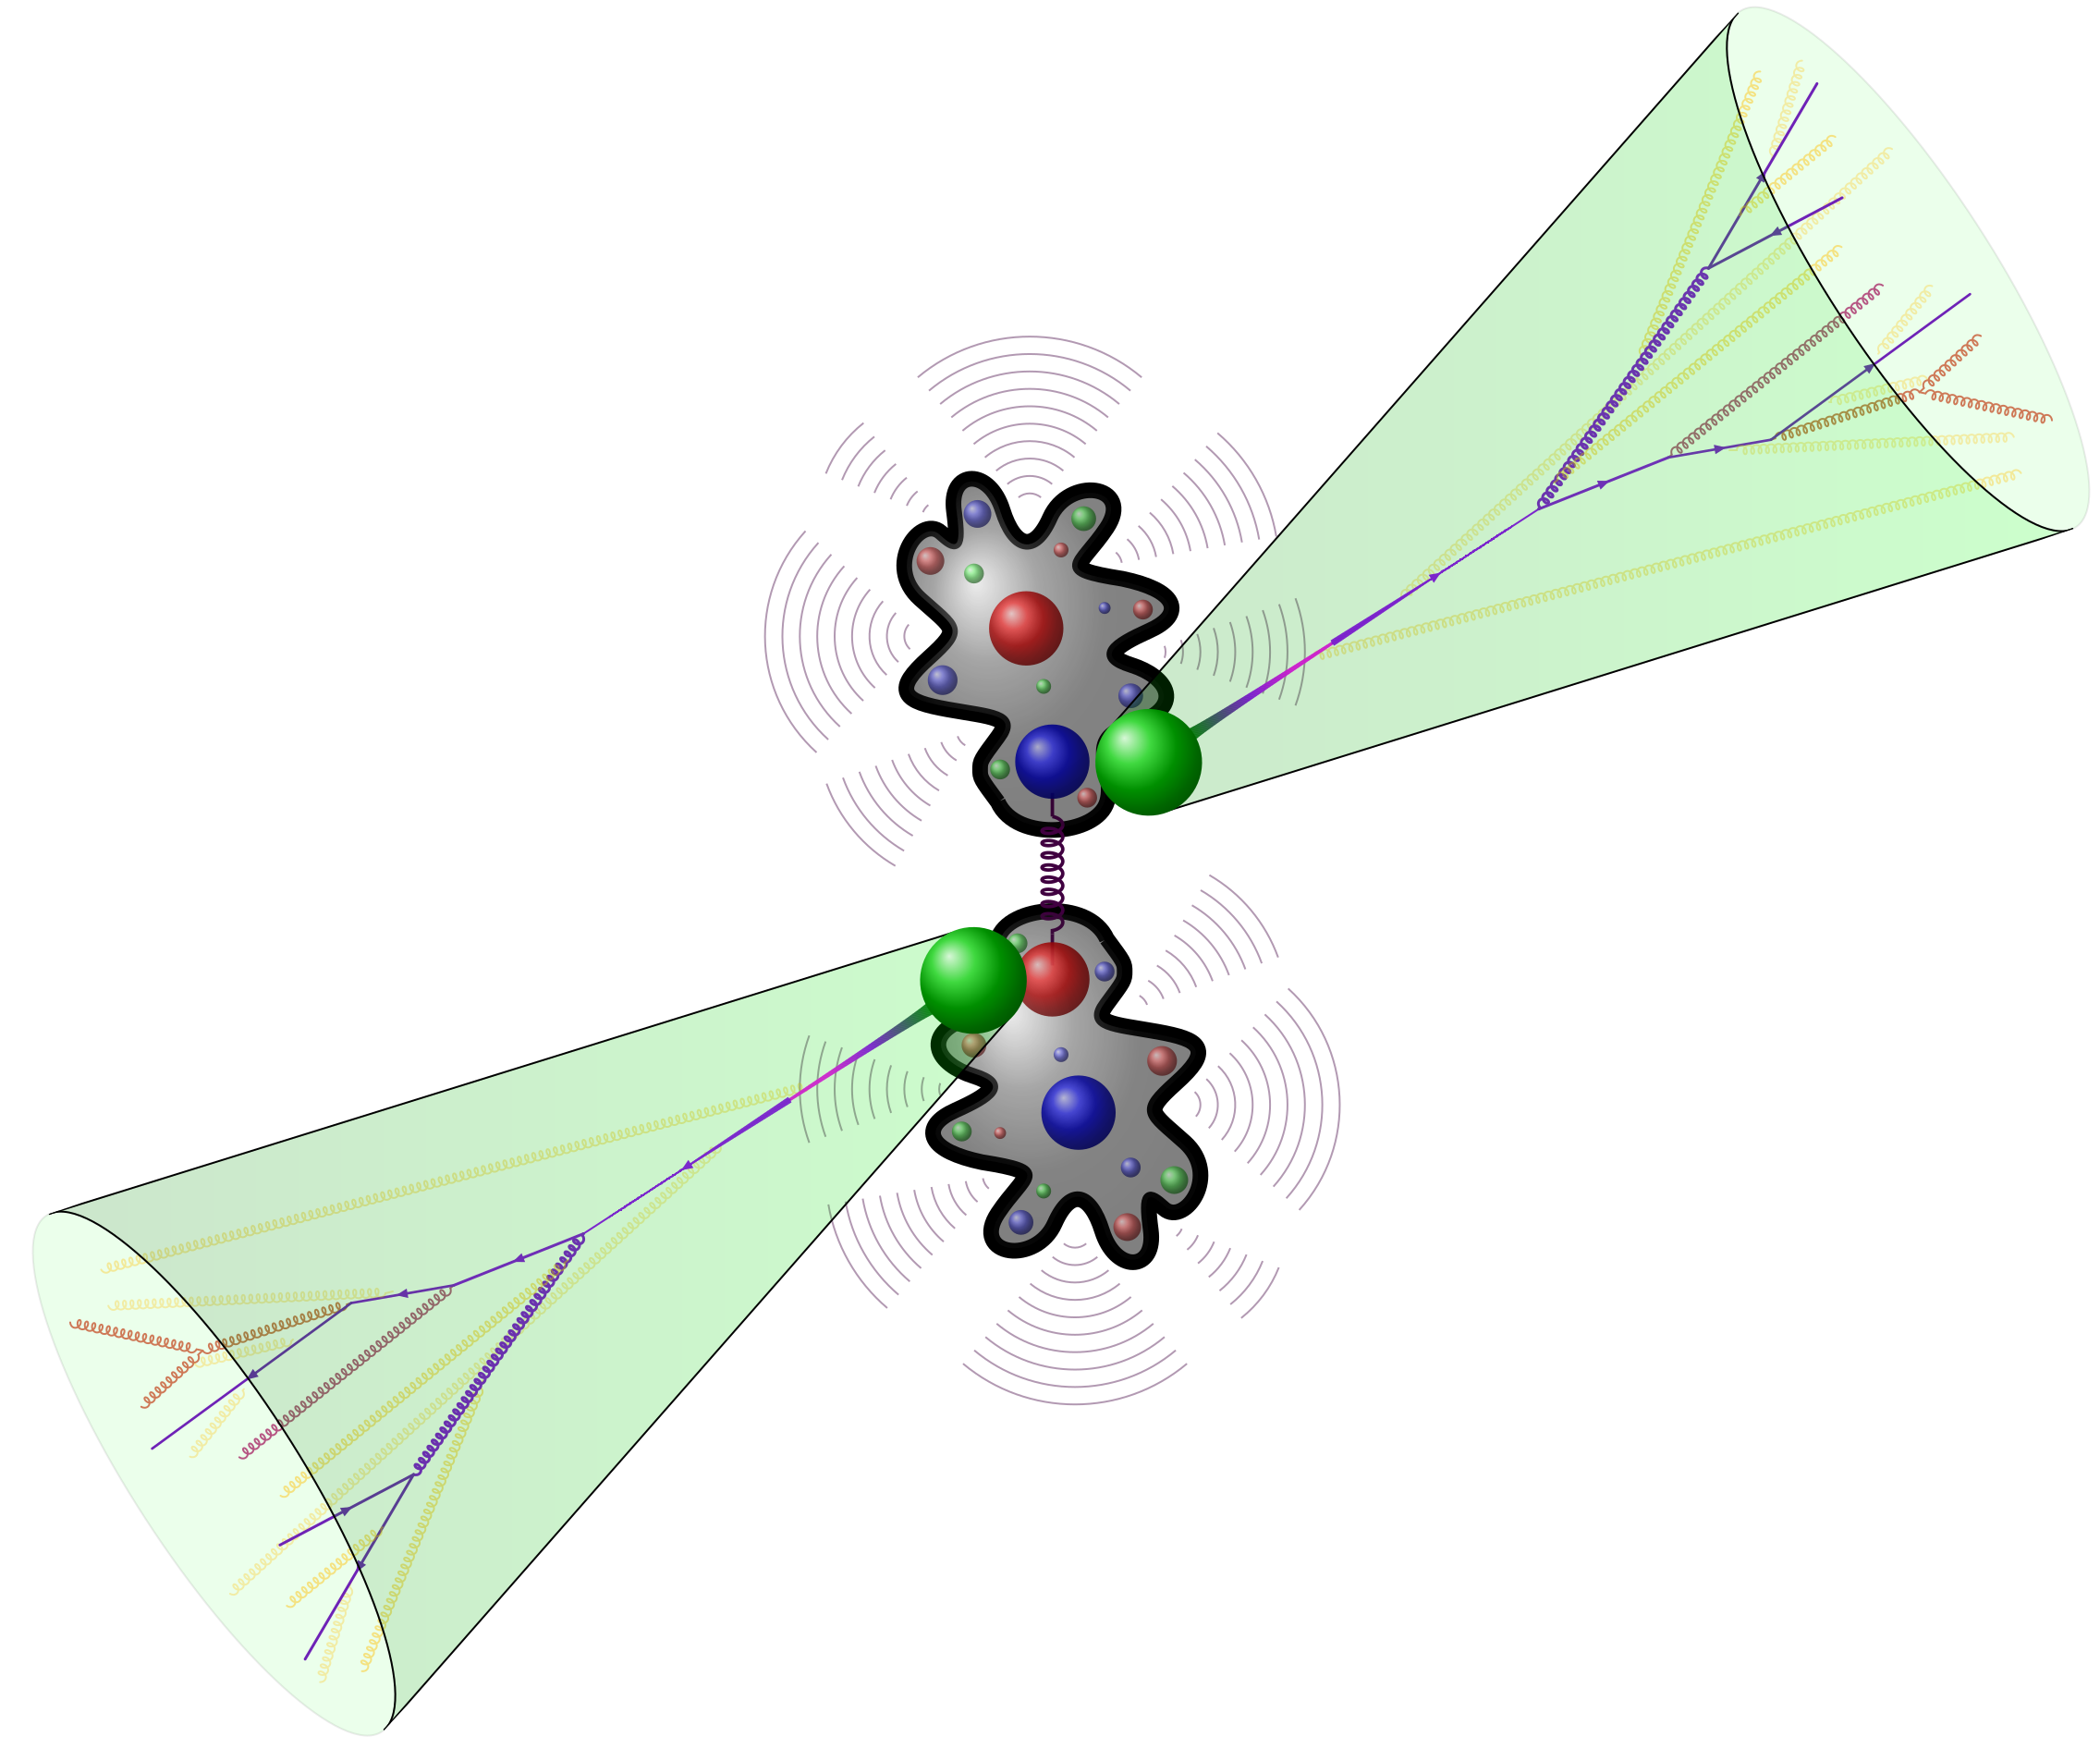
\includegraphics[width=0.48\textwidth]{figures/misc/ue-jets}
        \label{fig:app-ue}
    }
    \subfloat[]{
        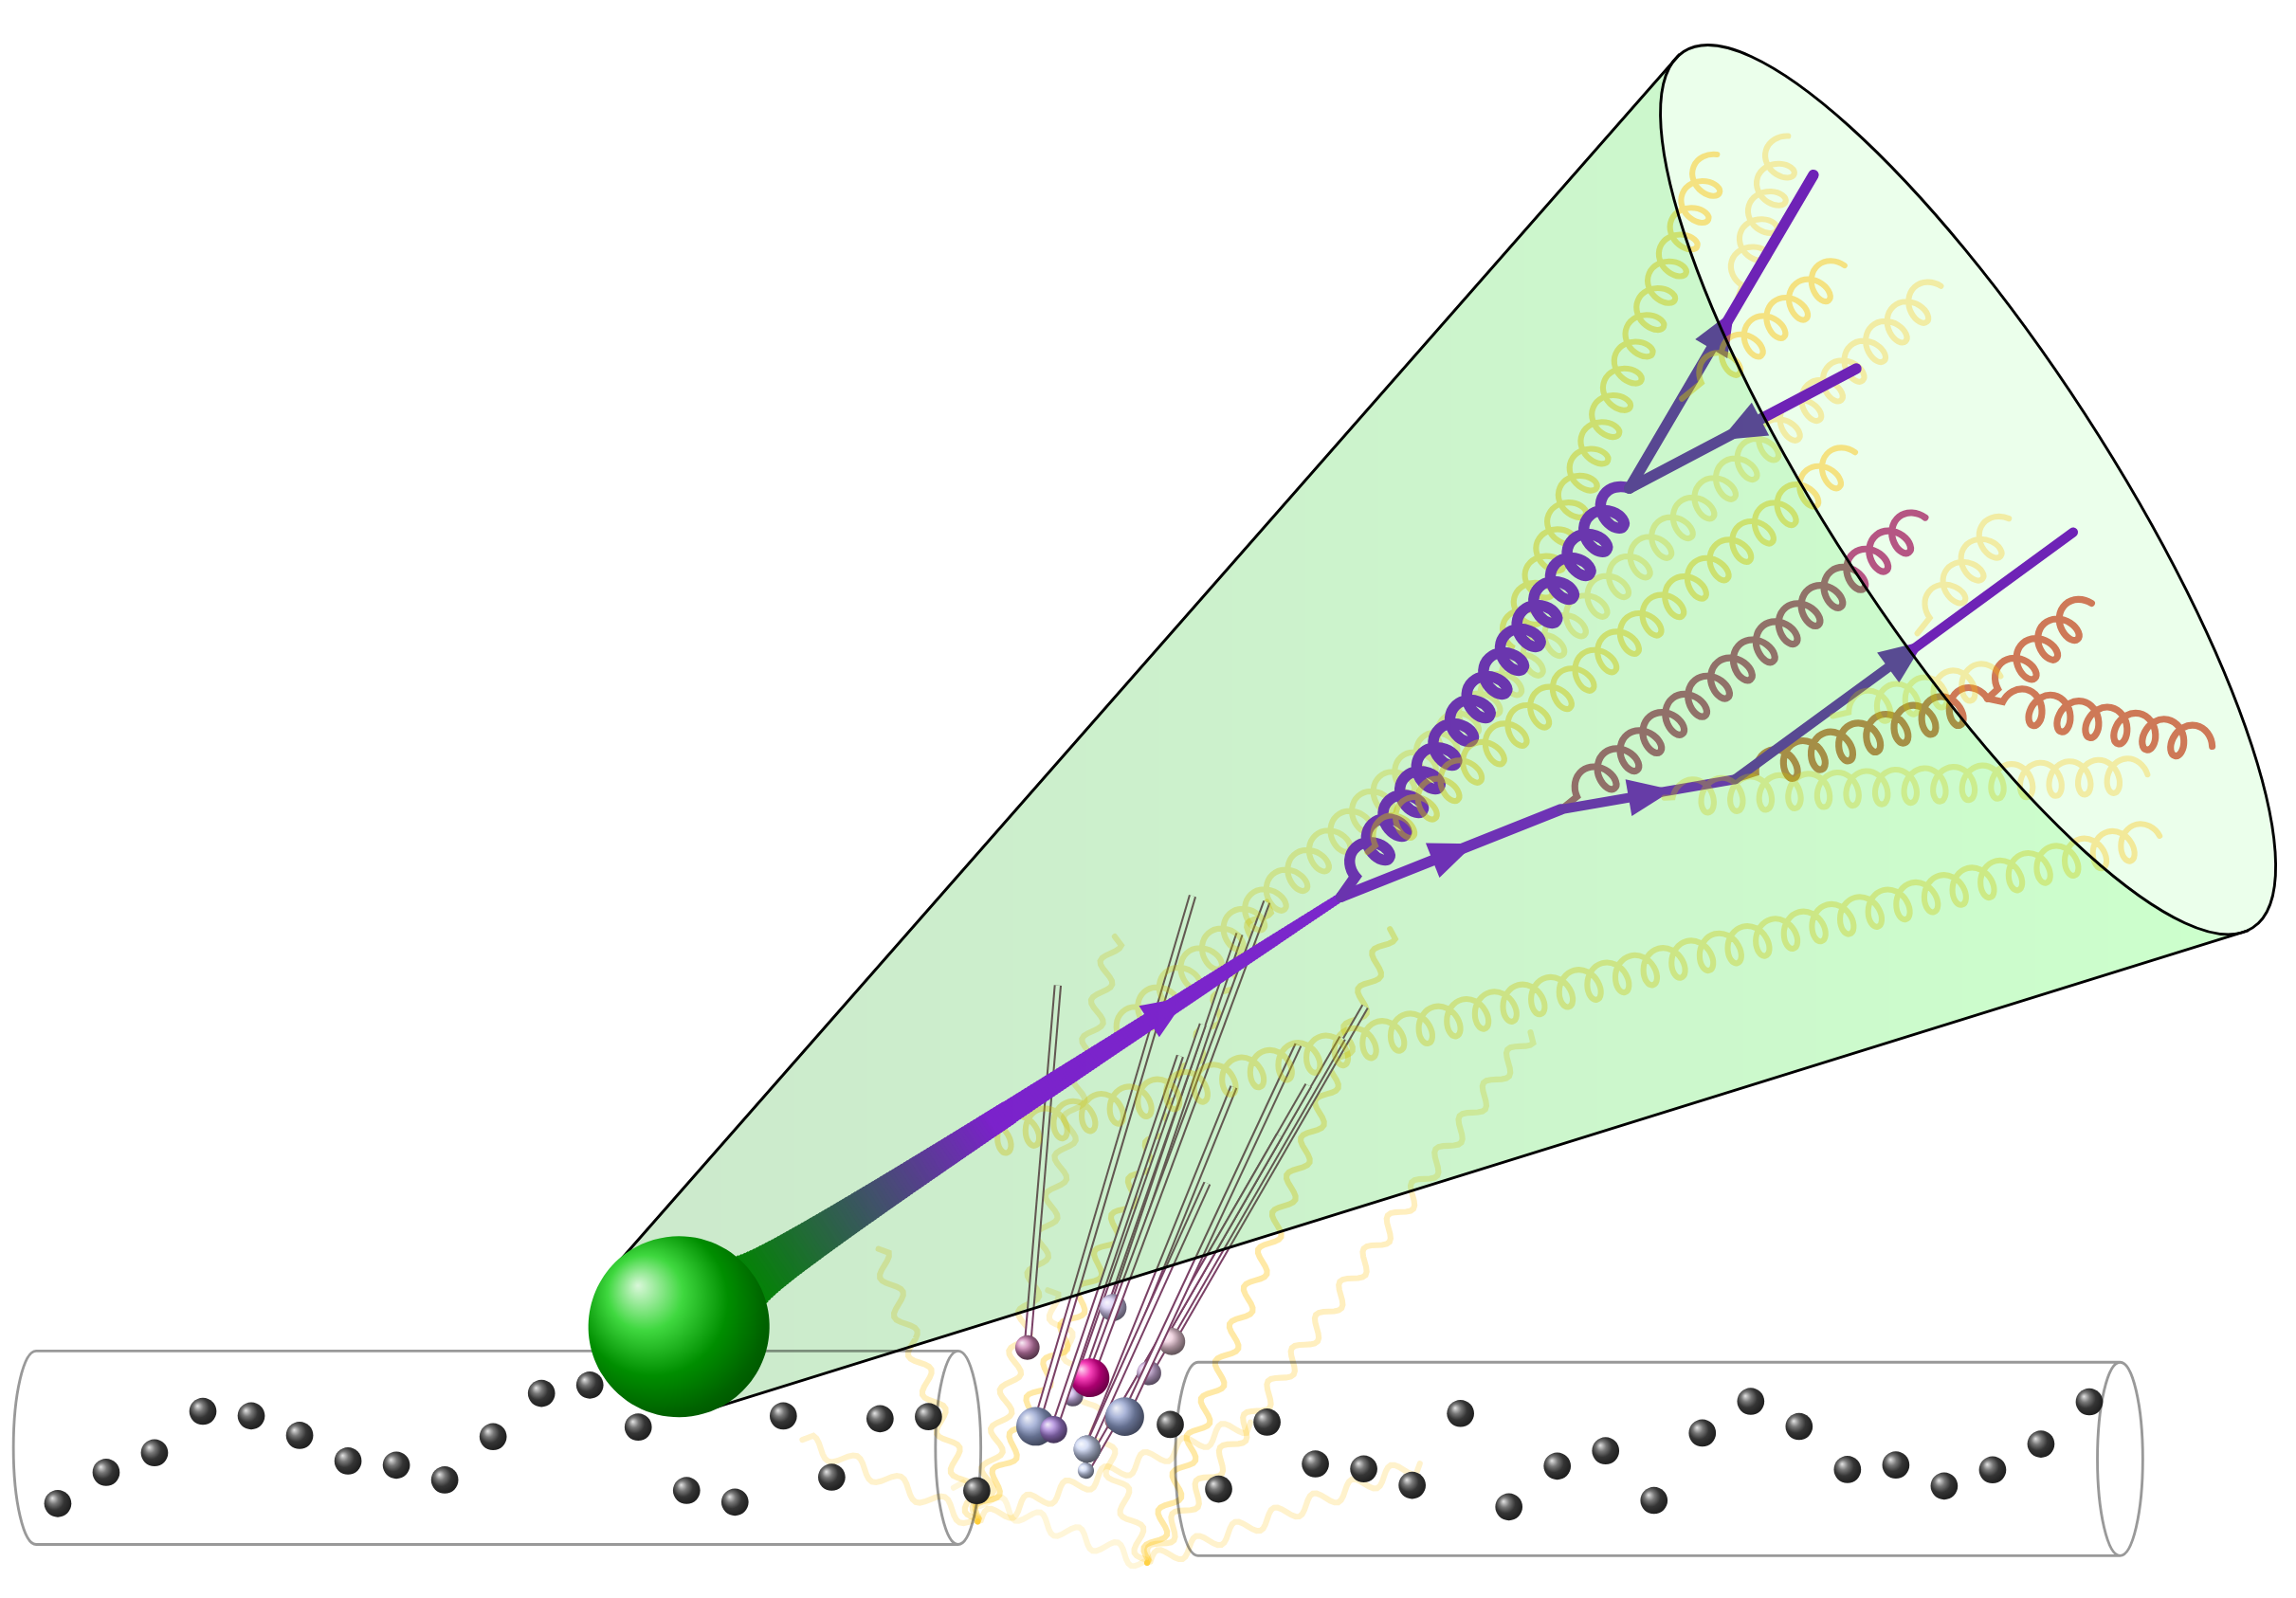
\includegraphics[width=0.48\textwidth]{figures/misc/pu-jet}
        \label{fig:app-pu}
    }
    \caption[Visualizations of additive contamination in particle collisions.]{Visualizations of important sources of additive contamination in particle collisions:
    %
    \hyperref[fig:app-ue]{(a)}
    \glslink{ue}{the underlying event (UE)}, described theoretically through additional interactions from partons which are not directly involved in a hard scattering process, and
    %
    \hyperref[fig:app-pu]{(b)}
    \glslink{pileup}{pileup (PU)}, or radiation from lower energy scatterings of \textit{additional} protons not directly involved in a primary hard scattering.
    }
    \label{fig:app-additive-contamination}
\end{figure}


The \glslink{ue}{underlying event (UE)} (see \Fig{app-ue}) is a theoretical source of additive contamination in hadronic collisions whose behavior must be modelled for accurate predictions of jet substructure.
%
The first-principles framework of \gls{ue} is an area of active research, but in this thesis we use the well-understood and highly successful framework of \textit{\glslink{mpi}{multiple parton interactions (MPI)}} in \gls{pythia}.

\begin{definitionbox}{Underlying Event}{ue}
    \vocab{\glslink{ue}{The underlying event (UE)}} is radiation produced in a high-energy hadron collision that is not directly related to the hard scattering process that produces the primary partons or jets.
    %
    The dominant model of \gls{ue} is the \vocab{\gls{mpi}} model of \gls{pythia}.

    In the context of hadronic collisions in \gls{pythia}, \glslink{mpi}{multiple parton interactions} occur when, rather than the collision involving only one parton from each hadron, the more detailed inner structure of the hadrons involving multiple partons is taken into account.
    %
    \gls{mpi} refers to the additional scatterings of these multiple partons (in principle described by generalized \(n\)-parton distribution functions, though the rarity of these additional scatterings means that only 2-parton distribution functions are needed in practice).
\end{definitionbox}



\remark{mpi}{
    The \gls{mpi} model of \gls{pythia} also combines the multiple-parton-scattering model described above with insights from a theoretical description of all-orders effects in scattering (called Regge-Gribov theory, after its creators \cite{Gribov:1967vfb}) in which ``cut pomerons'', beyond the scope of this thesis, contribute to hadronic cross sections through the production of a large number of low-energy gluons.
    %%
    %An understanding of the ideas of Regge-Gribov theory in effective field theory is an area of ongoing research which, to my knowledge, is spearheaded by the framework of Glauber \gls{scet} (see, for example, discussion in Secs. 7.2, 8, and 9, of \Reff{Rothstein:2016bsq}, as well as interesting discussions in \Reffs{Moult:2022lfy,Gao:2024qsg,Gao:2024fyz}).
}


\remark{}{
    The number of multiple-parton interaction vertices in \gls{pythia} is taken to be Poisson-distributed.
    %
    Furthermore, the radiation produced by multiple-parton scatterings is, when averaged, roughly uniform in the rapidity-azimuth plane.
    %
    These simple features allow for the development of tractable phenomenological models for certain features of \gls{ue}.
    %
    A particularly elegant characterization is given by \Reff{Cacciari:2009dp}.
    %
    Among other characterizations of the expected phenomenological behavior of \gls{ue}, they are able to explicitly derive an estimate of the distribution of transverse momenta due to \gls{ue} in a given area of the rapidity-azimuth plane, assuming a Poisson-distributed number of outgoing particles from \gls{ue} and an exponential distribution for their transverse momenta.
    %
    Under these assumptions, they find (in \href{https://arxiv.org/pdf/0912.4926\#page=7}{Section 3.1}, see also \href{https://arxiv.org/pdf/0912.4926\#page=35}{Appendix A} and \href{https://arxiv.org/pdf/0912.4926\#page=7}{footnote 2}) the surprisingly compact result
    \begin{align}
        \frac{\dd P}{\dd p_T^{\rm(UE)}}(A)
        =
        e^{-\nu A}
        \le(
            \delta\le(p_T^{\rm(UE)}\ri)
            +
            e^{-p_T^{\rm(UE)}/\mu}
            \sqrt{\frac{A \, \nu}{p_T^{\rm(UE)}\, \mu}}
            I_1\le(2\sqrt{\frac{A\,\nu\, p_T^{\rm(UE)}}{\mu}}\ri)
        \ri)
        \,,
    \end{align}
    where $I_1$ is a modified Bessel function (of the first kind), \(\nu\) is the parameter which governs the average of the Poisson-distributed number of particles per unit area (\(\nu \sim 5\) is the realistic value they give for \gls{ue} at the LHC), and \(\mu\) is a parameter governing the average of the exponentially-distributed transverse momentum of each individual particle (they give \(\mu \sim\) 0.4 GeV, which they find corresponds to an average \(p_T\)-per-area of about 2 GeV).
    %
    Unfortunately, this elegant result does not make further appearances in this thesis.
}

In this thesis, we look at examples in which we characterize the effects of the underlying event on the distribution of collider observables.
%
A more rigorous analyst would also quantify the \textit{uncertainties} in distributions \textit{due to the modelling of the underlying event}.
%
Analyses of uncertainties due to \gls{ue} modelling -- as performed in experimental analyses -- involves at least the two following steps:
\begin{itemize}
    \item
        \textbf{Reweighting:} (also important for \gls{pileup})

        We have theoretical expectations for the distribution number of multiple-parton interactions, \(N_\text{UE}\), associated with collision events at a certain scale, but we want to quantify our uncertainty about the precise form of the \(N_\text{UE}\) distribution.
        %
        This is achieved by \textit{re-weighting} events -- i.e. re-weighting their contributions to histograms -- based on the effective value of \(N_\text{UE}\).
        %
        We give a simplistic description of re-weighting, in which we assume we have access directly to \(N_\text{UE}\), in Example \ref{ex:reweighting-ue} below.
        %
        In practice, however, re-weighting is performed by re-weighting events by a function of collision parameters that are closely related to \gls{ue}, rather than \(N_\text{UE}\) itself.
        %
        In particular, when simulating \gls{ue} with \gls{pythia}, one can keep track of scales used by the shower algorithm to generate initial-state radiation (ISR) and final-state radiation (FSR) for each collision.
        %
        These are are also correlated with the number \(N_\text{UE}\) of multiple-parton interactions.
        %
        By re-weighting events based on the ISR and FSR scales of the shower, one can effectively change the distribution of \(N_\text{UE}\) associated with the generated events.


    \item
        \textbf{Changing tunes:}

        To characterize uncertainties in other parameters of the \gls{ue} model (usually reserved only for precision measurements), one chooses several, previously tuned/validated values of particular \gls{pythia} parameters controlling \gls{ue} behavior -- called the \vocab{\gls{pythia} tune} -- and examine the differences in the distributions obtained with different tunes.
\end{itemize}

\remark{}{
    In this thesis, we perform no re-weighting, and only present results obtained with the default Monash tune of \gls{pythia} \cite{Skands:2014pea}.
    %
    The \gls{pythia} tune often preferred in experimental analyses is the CP5 tune introduced by the CMS experiment \cite{CMS:2022awf}.
}


\begin{example}
    \label{ex:reweighting-ue}
    While in practice one re-weights based on the ISR and FSR scales recorded by \gls{pythia}, let us imagine a simpler situation in which we can directly keep track of the number of underlying event collisions \(N_\text{UE}\).
    %
    We imagine that \(N_\text{UE}\) is Poisson distributed with some mean \(\nu\);
    %
    however, uncertainties in \(\nu\) lead to uncertainties in distributions obtained with \gls{pythia}.
    %
    If we want to understand the effect of uncertainties in \(\nu\) on a histogram describing the distribution of a collider variable \(X\), we can \textit{re-compute} the distribution of \(X\), but with \vocab{re-weighted} contributions from from events with different values of \(N_\text{UE}\):
    %
    each event fills a histogram bin with a weight \(w(N_\text{UE})\), rather than one as in the original histogram for \(X\).
    %
    The weight is chosen such that the \textit{effective} number of of multiple-parton interactions is Poisson distributed with a \textit{new} mean \(\nu' \neq \nu\), e.g.
    \begin{align}
        \label{eq:re-weighting-ue}
        \nu'
        =
        \le\langle N_\text{UE}\ri\rangle_\text{re-weighted}
        =
        \frac{
            \sum_{\text{events } i}
            N_i w(N_i)
        }{
            \sum_{\text{events } i}
            w(N_i)
        }
        \neq
        \nu
        \,,
    \end{align}
    where \(N_i\) is the number of multiple-parton interactions in event \(i\).
\end{example}

\begin{exercise}
    Design a re-weighting scheme:

    Given a distribution Poisson($\nu$) with mean \(\nu\), find a weight function \(w_{\nu \to \nu'}(N)\) such that a set of data \(\{N_i\}\) drawn from Poisson($\nu$), re-weighted by \(w_{\nu \to \nu'}(N)\), behaves as if it were drawn from the distinct Poisson distribution Poisson($\nu'$).

    \vspace{7pt}

    \texttt{(Hint:)}
    %
    Your result should be a simple ratio.
\end{exercise}


% \begin{figure}[]
%     \centering
%     \includegraphics[width=0.8\textwidth]{example-image-a}
%     \caption{{Re-weighting}}
%     \label{fig:reweighting}
% \end{figure}


An important experimental source of additive contamination in particle collisions is \glslink{pileup}{pileup (PU)} (see \Fig{app-pu}).
%
Pileup occurs when radiation from an unrelated collision is detector together with the jets, or other high-energy information, from a collision of interest.

Unfortunately, pileup is a necessary feature of modern particle collisions if we want to generate enough collision events to learn about the universe.
%
When colliding protons at the LHC, for example, the vast majority of collisions yield ``uninteresting'' results -- that is, results which do not produce the high-energy jets or other high-energy phenomena for which we need collision experiments.
%
In order to see and test interesting physical results, such as the production of the Higgs boson, we therefore need to collide a huge number of protons.
%
By applying very strong and precise electromagnetic fields, we are able to line up a huge number of protons into a \textit{bunch};
%
particle physics experiments then accelerate two bunches of protons towards each other so that we can observe the results of many collisions.

When two bunches cross, we are more likely to see an interesting particle collision occur -- for example, one with high energy jets.
%
However, the interactions of other protons in each bunch produces produce additional final-state particles included in our experimental results.


\begin{definitionbox}{Pileup}{pileup}
    \vocab{\glslink{pileup}{Pileup (PU)}} refers to the additional interactions in a hadron collision due to multiple collisions occurring nearly simultaneously within the same bunch crossing.
    %
    These additional collisions are not directly related to the hard scattering process of interest but nonetheless interfere with measurements of the primary hard-scattering event, especially in high-luminosity environments.
\end{definitionbox}


\remark{}{
    Since the pileup collisions are approximately un-correlated, the number of pileup events \(N_\text{PU}\) polluting a collision of interest is approximately Poisson distributed.
    %
    There are several methods to experimentally determine the distribution of the number of pileup vertices.
    %
    One is by using known properties of the cross-section associated with \gls{pileup} interactions, \(\sigma_\text{PU}\), and the luminosity of the experiment, \(\mathcal{L}\), to write \(\le\langle N_\text{PU}\ri\rangle = \sigma_\text{PU} \mathcal{L}\).
    %
    Another is by measuring the distribution of \vocab{primary vertices} measured in a particle collision.
    %
    Primary vertices are points from which sets of final-state particles seem to emerge, based on more detailed experimental reconstruction, so \(N_\text{PU} = N_\text{primary} - 1\).%
    \footnote{
        Primary vertices lie only along the axis of the colliding proton beams -- the \(z\) axis -- and are separated in the \(z\) direction.
        %
        \emph{Secondary vertices} -- vertices associated with the decay of a particle emerging from a primary vertex -- would instead be located away from the beam (i.e. with \(x, y \neq 0\)).
    }
    %
    Yet another is by measuring the distribution of transverse momentum per unit rapidity-azimuth area and relating this to the number of pileup events;
    %
    since the transverse momentum produced a pileup event is, on average, uniform in the rapidity-azimuth plane \cite{Soyez:2018opl,Monk:2018clo,Sjostrand:1987su,Sjostrand:2014zea,Dasgupta:2007wa,Kirchgaesser:2020poq,Moraes:2007rq,CDF:2015txs,Larkoski:2021hee,Baron:2020xoi,Marzani:2017kqd}, we expect \(p_T / A \propto N_\text{PU}\) for any given event.
}


\glslink{pileup}{Pileup} events are modelled in both theoretical and experimental contexts by generating \vocab{minimum bias events} -- roughly, events which pass a bare minimum of experimental cuts -- using \gls{pythia}.
%
The number \(N_\text{PU}\) of pileup collisions to be added to the simulated collision of interest is drawn from the appropriate distribution, such as the experimentally measured distribution of \(N_\text{primary} - 1\), or a Poisson distribution with the experimentally realistic mean \(\le\langle N_\text{PU}\ri\rangle \sim 20 - 30\) \cite{Soyez:2018opl}.
%
Then, this number of simulated minimum bias events are generated (or loaded from an existing database), and their final-state particles are added to the set of final state-particles of the simulated collision of interest;
%
the resulting set of final-state particles forms the simulated event together with its simulated pollution.

\remark{}{
    Just as in the case of \gls{ue}, uncertainties in the average number of pileup events, or the pileup distribution more generally, are captured in more detailed analyses by re-weighting (though we do not pursue that level of rigor in this thesis).
    %
    Re-weighting to estimate the effects of varying the \gls{pileup} distribution, however, is simpler in practice than re-weighting for \gls{ue};
    %
    since we may directly keep track of the number of minimum bias events we add to every collision, we may re-weight events directly by a function only of \(N_\text{PU}\) (rather than by a function of indirect probes of \(N_\text{PU}\), as in the case of ISR and FSR scales providing indirect probes of \(N_\text{UE}\)).
}

Pileup can significantly affect jet measurements and leads to difficulties in extracting information about jet substructure.
%
\glslink{pileup}{pileup} and the principles of \glslink{pu-mitigation}{pileup mitigation} will play an important role in our pursuit of jet substructure observables which are insensitive to the effects of low-energy pollution.

\begin{definitionbox}{Pileup Mitigation}{pu-mitigation}
    \vocab{\Gls{pu-mitigation}} refers to any strategy for reducing the impact of \glslink{pileup}{pileup} events on hadronic collisions in high-luminosity environments, usually by separating the jets generated by a primary hard scattering from unwanted pileup contributions.
\end{definitionbox}

In the next chapter, we will make the unusual choice to merge the terms \gls{pu-mitigation} and \gls{jet-grooming}.
%
As we discuss in the next chapter, jet grooming is any method which modifies the constituents of a jet in order to reduce the effects of low-energy pollution.
%
Therefore, we describe \gls{pu-mitigation} as a type of \gls{jet-grooming} which aims specifically to remove \gls{additive-contamination}.
\end{subappendices}



% %%%%%%%%%%%%%%%%%%%%%%%%%%%%%%%%%%%%
% Problems
% %%%%%%%%%%%%%%%%%%%%%%%%%%%%%%%%%%%%
\begin{problems}

\makeprob{The No-Emission Probability (Sudakov Form Factor)}{no-emission}{
    Let \(\Pi_i(m^2 \leftarrow Q^2)\) indicate the probability that, within a partonic cascade initiated by a parton of flavor \(i\) and virtuality \(Q\), that there is no pairwise emission of partons with a mass larger than \(m\);
    %
    this is sometimes called a \vocab{Sudakov form factor} or a \vocab{no-emission probability}.

    \begin{enumerate}[label=\alph*)]
        \item
        Using the strongly-ordered limit, argue that
        \begin{align}
            \Pi_i(m^2)
            \approx
            \exp[
                -
                \,
                \int \dd z
                \,\,
                4\as
                \,
                \sum_j p_{j \leftarrow i}(z)
                \,
                \int \frac{\dd \theta}{\theta}
                \,\,
                \,
                \Theta(z\theta^2 > m^2)
            ]
            \,,
        \end{align}
        and identify where the strongly-ordered limit appears in your analysis.

        Repeat your analysis to calculate the probability that there is no pairwise emission of partons with an \textit{angularity} (\(z_\text{soft}\,\theta^\varsigma\)) less than \(e_\varsigma\);

        \item
        Explicitly compute the analytic form of the LL no-emission probability for angularities that you derived in integral form in (a).
    \end{enumerate}
}




\makeprob{The Algorithms for Generating Partonic Emissions}{veto-algorithm}{
    When simulating the partonic cascade, the complicated form of the splitting functions and running coupling make analytic results more difficult to obtain even for simple quantities (such as the \gls{parton-to-parton} of \Sec{p2p-fragmentation}).
    %
    To solve more complicated problems, it is common to use numerical parton showers and random number generation to simulate the generation of emissions in the partonic cascade.
    %
    In this problem, we explore the basics of some simple sampling techniques.


    \begin{enumerate}[label=\alph*)]
        \item
        \vocab{Inverse transform sampling} can be used when we have a probability distribution for a random variable \(X\) whose cumulative distribution \(F(X)\) has a known inverse \(F^{-1}(y)\).
        %
        Inverse transform sampling leverages that it is relatively simple to sample a random variable \(U\) which is uniformly distributed from 0 to 1, and relies on the fact that \(F^{-1}(U)\) can be used to obtain the probability distribution of \(X\).

        \textit{Show that \(F^{-1}(U)\) has the same cumulative probability distribution as \(X\) and use this fact to justify inverse transform sampling.}


        \item
        The \vocab{\gls{veto-algorithm}} allows us to sample from an exponential cumulative distribution of the form
        \begin{align}
            \Pi_f(x\,|\,T) = \exp\le[-\int_x^T \, \dd x' \, f(x')\ri]
            \,,
        \end{align}
        where \(f(x')\) is known and positive semi-definite, but its integral may not be known (this is intentionally reminiscent of \Prob{no-emission}).
        %
        In particular, the veto algorithm, much like the accept-reject algorithm, depends on a reference probability distribution;
        %
        in this case, the reference probability distribution also has an exponential cumulative form, \(\Pi_g(x | T)\), has the probability distribution \(g(x) \Pi_g(x | T)\), and must satisfy \(f(x) \leq g(x)\) for all \(x\).

        The veto algorithm is represented graphically through the flow of code
        \begin{center}
            \raisebox{-\height}
            {
            \begin{tikzpicture}
                \node[rectangle, minimum width=1.0cm, minimum height=0.75cm, thin, draw=black] (sample) at (0, 3.4) {Sample $x$ from $g(x) \, \Pi_g(x \, | \, T)$};
                \node[rectangle, minimum width=1.0cm, minimum height=0.75cm, thin, draw=black] (accept) at (0, 1.7) {Accept trial with probability $\frac{f(x)}{g(x)}$};
                \node[rectangle, minimum width=1.0cm, minimum height=0.75cm, thin, draw=black] (done)   at (0, 0.0) {Done};
                \node[rectangle, minimum width=1.0cm, minimum height=0.75cm, thin, draw=black] (veto)   at (3.6, 2.8) {Set $u = t$};


                \draw[black, line width=2pt, -Stealth] (sample) to [out=270,in=90] (accept);
                \draw[red!80!black, line width=2pt, looseness=2.3, -Stealth]   (accept) to [out=0,in=270](veto);
                \draw[red!80!black, line width=2pt, looseness=1.0, -Stealth] (veto) to [out=90,in=0](sample);
                \draw[green!70!black, line width=2pt, -Stealth] (accept) to [out=270,in=90](done);


                \node[green!50!black] at (1.2, 0.8) {If \textbf{Accept}};
                \node[red!50!black] at (5.0, 1.3) {Otherwise (\textbf{Veto})};
            \end{tikzpicture}
        }
    \end{center}

    \textit{Show that the \gls{veto-algorithm} described by the graphic above accurately samples from the desired probability distribution.}
    \end{enumerate}

    \noindent
    (\texttt{Note:} Adapted directly from \Reff{Bierlich:2022pfr}, whose section 2.2 is a wonderful resource for learning about sampling and Monte Carlo algorithms)
}


\makeprob{\(\star\) A Numerical Parton Shower \(\star\)}{parton-shower}{
    Using the results of \Probs{no-emission}{veto-algorithm}, write pseudocode for a parton shower algorithm which generates emissions ordered by angularity, i.e. such that the angularity of any emission is smaller than that of its parent.
}


\makeprob{Recursive Fragmentation Functions}{p2p-fragmentation}{
    As in \Sec{p2p-fragmentation}, let \(F_{j\leftarrow i}(z\,|\,\rsub \leftarrow \Rjet) \,\, \dd z\) denote the probability of finding a parton of flavor \(j\) at an angular scale \rsub, with momentum fraction between \(z\) and \(z + \dd z\) of an initiating parton \(i\) measured at an angular scale \Rjet.

    \begin{enumerate}[label=\alph*)]
        \item
            Derive the recursive fragmentation formula,
            \begin{align}
                \label{eq:feynman_field_fragmentation_formula}
                F_{j\leftarrow i}(z\,|\,\rsub\leftarrow\Rjet)
                \,\,
                =&
                \,\,
                \delta(1-z) \, \delta_{ij}
                \\
                \notag
                &
                \,
                +
                4
                \,
                \int_{\rsub}^{\Rjet} \frac{\dd\theta}{\theta} \,
                \int_z^1 \frac{\dd y'}{y'} \,
                    \,
                    a_s
                    \,
                    \sum_{k'}
                    F_{j\leftarrow k'}(z/y'\,|\,\theta\leftarrow\Rjet)
                    \,
                    p_{k' \leftarrow i}(y')
                \,,
            \end{align}
            through physical intuition.

        \item
            Does \Eq{feynman_field_fragmentation_formula} have the correct behavior at \(\Rjet = \rsub\)?

        \item
            Show that the recursive fragmentation formula also implies the DGLAP equations of \Eq{dglap-equations-parton-shower}, which were derived through a more complete parton shower approach in \Sec{p2p-fragmentation}.
    \end{enumerate}
}


\makeprob{\(\star\star\) Multiple Emissions \(\star\star\)}{multiple-emissions}{
    \begin{enumerate}[label=\alph*)]
        \item
            Write an expression, in terms of an infinite sum over products of phase space factors, for the cumulative distribution of an additive observable \(X\);
            %
            do \textit{not} use the approximation that the value of \(X\) is set by a single emission discussed in \Prop{ll-additive} and \Sec{ll-substructure-diagrams}.

        \item
            By taking a Laplace transform, performing a sum, and taking an inverse Laplace transform, show that the cumulative distribution for the additive observable \(X\) can be written in the form
            \begin{align}
                \Sigma(x)
                \approx
                \frac{\exp[-H(x)]}{\Gamma\le(1 + H'(x)\ri)}
                \,,
            \end{align}
            up to terms of \(\mathcal{O}(H''(x))\), where \(H'(x) := -\dd H(x) / \dd \log(x)\).
            %
            What is \(H(x)\)?

            \texttt{(Hint:)} You may need the formula \(\int_{c-i\infty}^{c+i\infty} \frac{\dd y}{2 \pi i y} e^y y^{-A} = 1/\Gamma(1 + A)\) for the inverse Laplace transform of \(e^y y^{-1-A}\);
            %
            this can be found e.g. in \href{https://arxiv.org/pdf/1809.03933\#page=5}{Lemma 2.1 of} \Reff{schmidt2019shortnoteintegraltransformations}, or \href{https://univ.jeanpaulcalvi.com/Posters/ConfAuchWeb/abramovitz2.pdf\#section.5.9}{Section 5.9 of} \Reff{822801}.

        \item
            Argue that, for small \(x\), \(H(x)\) is approximately given by \(R_X(x)\), and show that this reproduces the correct leading logarithmic features derived in \Sec{ll-substructure-diagrams}.

        \item
            When \(X\) is an angularity, show that
            \begin{align}
                H(x) = R_X(x) + \gamma_E R'(x)
                \,,
            \end{align}
            and therefore that the cumulative distributions of angularities, when multiple emissions are included, take the form
            \begin{align}
                \Sigma(x) \approx \frac{e^{-R(x) - \gamma_E R'(x)}}{\Gamma\le(1 + H'(x)\ri)}
                \,.
            \end{align}

        \item
            Justify our neglect of the terms of \(\mathcal{O}(H''(x))\).
    \end{enumerate}
}




\makeprob{\(\star\) Angularities at modified leading-logarithmic accuracy \(\star\)}{mll-angularities}{
    Using the result of \Prob{multiple-emissions}, and taking into account running coupling effects, write an analytic expression for the MLL cumulative distribution for angularities in jets initiated by a parton of flavor \(i\), and show that it recovers the correct LL result in the limit \(\alphas\to0\).
    %
    Recall that the MLL result should include running coupling effects, multiple emissions, and non-singular pieces of the splitting functions.
    %
    If you are brave, you may also freeze the coupling below a non-perturbative scale.

    \texttt{(Hint:)} Luckily, as discussed at the end of \Sec{ll-substructure-diagrams}, you may assume all contributions are from the primary branch of the jet, so that you will only need to use the form of a single splitting function, \(p_{i g \leftarrow i}(z)\), for each \(i\).
}





\vspace{10pt}
\hrule
\vspace{10pt}


\section*{Problems on the Mellin Transform}


\makeprob{Mellin Convolution Theorem}{mellinconvolution}{ Prove the Mellin Convolution Theorem of Proposition~\ref{prop:mellin-convolution-app}.  }


\makeprob{Mellin Convolution Theorem II}{mellinconvolution2}{
    There is another, related convolution in the context of Mellin transforms.
    %
    Consider the new convolution
    \begin{align}
        (f \circ_{\mc M} g)(x)
        =
        \int_0^\infty\,\dd\xi f(x\,\xi) g(\xi)
        \,.
    \end{align}
    Show that the Mellin transform of this convolution is
    \begin{align}
        \mathcal{M}[f \circ_{\mc M} g](s)
        \,
        =
        \,
        \mathcal{M}[f](s) \, \mathcal{M}[g](1-s)
        =:
        \hat{f}(s) \, \hat{g}(1-s)
        \,.
    \end{align}
}
% \begin{exercise}
%     {BFKL... turn to problem}
    % https://www.hep.phy.cam.ac.uk/theory/webber/QCDlect3.pdf#page=22
% \end{exercise}


% Multiplicity... similar to the techniques of jet calculus, but I first saw it in...
%https://arxiv.org/pdf/1704.06266

\end{problems}
